% Options for packages loaded elsewhere
\PassOptionsToPackage{unicode}{hyperref}
\PassOptionsToPackage{hyphens}{url}
\PassOptionsToPackage{dvipsnames,svgnames,x11names}{xcolor}
%
\documentclass[
  letterpaper,
  DIV=11,
  numbers=noendperiod]{scrreprt}

\usepackage{amsmath,amssymb}
\usepackage{iftex}
\ifPDFTeX
  \usepackage[T1]{fontenc}
  \usepackage[utf8]{inputenc}
  \usepackage{textcomp} % provide euro and other symbols
\else % if luatex or xetex
  \usepackage{unicode-math}
  \defaultfontfeatures{Scale=MatchLowercase}
  \defaultfontfeatures[\rmfamily]{Ligatures=TeX,Scale=1}
\fi
\usepackage{lmodern}
\ifPDFTeX\else  
    % xetex/luatex font selection
\fi
% Use upquote if available, for straight quotes in verbatim environments
\IfFileExists{upquote.sty}{\usepackage{upquote}}{}
\IfFileExists{microtype.sty}{% use microtype if available
  \usepackage[]{microtype}
  \UseMicrotypeSet[protrusion]{basicmath} % disable protrusion for tt fonts
}{}
\makeatletter
\@ifundefined{KOMAClassName}{% if non-KOMA class
  \IfFileExists{parskip.sty}{%
    \usepackage{parskip}
  }{% else
    \setlength{\parindent}{0pt}
    \setlength{\parskip}{6pt plus 2pt minus 1pt}}
}{% if KOMA class
  \KOMAoptions{parskip=half}}
\makeatother
\usepackage{xcolor}
\setlength{\emergencystretch}{3em} % prevent overfull lines
\setcounter{secnumdepth}{5}
% Make \paragraph and \subparagraph free-standing
\ifx\paragraph\undefined\else
  \let\oldparagraph\paragraph
  \renewcommand{\paragraph}[1]{\oldparagraph{#1}\mbox{}}
\fi
\ifx\subparagraph\undefined\else
  \let\oldsubparagraph\subparagraph
  \renewcommand{\subparagraph}[1]{\oldsubparagraph{#1}\mbox{}}
\fi

\usepackage{color}
\usepackage{fancyvrb}
\newcommand{\VerbBar}{|}
\newcommand{\VERB}{\Verb[commandchars=\\\{\}]}
\DefineVerbatimEnvironment{Highlighting}{Verbatim}{commandchars=\\\{\}}
% Add ',fontsize=\small' for more characters per line
\usepackage{framed}
\definecolor{shadecolor}{RGB}{241,243,245}
\newenvironment{Shaded}{\begin{snugshade}}{\end{snugshade}}
\newcommand{\AlertTok}[1]{\textcolor[rgb]{0.68,0.00,0.00}{#1}}
\newcommand{\AnnotationTok}[1]{\textcolor[rgb]{0.37,0.37,0.37}{#1}}
\newcommand{\AttributeTok}[1]{\textcolor[rgb]{0.40,0.45,0.13}{#1}}
\newcommand{\BaseNTok}[1]{\textcolor[rgb]{0.68,0.00,0.00}{#1}}
\newcommand{\BuiltInTok}[1]{\textcolor[rgb]{0.00,0.23,0.31}{#1}}
\newcommand{\CharTok}[1]{\textcolor[rgb]{0.13,0.47,0.30}{#1}}
\newcommand{\CommentTok}[1]{\textcolor[rgb]{0.37,0.37,0.37}{#1}}
\newcommand{\CommentVarTok}[1]{\textcolor[rgb]{0.37,0.37,0.37}{\textit{#1}}}
\newcommand{\ConstantTok}[1]{\textcolor[rgb]{0.56,0.35,0.01}{#1}}
\newcommand{\ControlFlowTok}[1]{\textcolor[rgb]{0.00,0.23,0.31}{#1}}
\newcommand{\DataTypeTok}[1]{\textcolor[rgb]{0.68,0.00,0.00}{#1}}
\newcommand{\DecValTok}[1]{\textcolor[rgb]{0.68,0.00,0.00}{#1}}
\newcommand{\DocumentationTok}[1]{\textcolor[rgb]{0.37,0.37,0.37}{\textit{#1}}}
\newcommand{\ErrorTok}[1]{\textcolor[rgb]{0.68,0.00,0.00}{#1}}
\newcommand{\ExtensionTok}[1]{\textcolor[rgb]{0.00,0.23,0.31}{#1}}
\newcommand{\FloatTok}[1]{\textcolor[rgb]{0.68,0.00,0.00}{#1}}
\newcommand{\FunctionTok}[1]{\textcolor[rgb]{0.28,0.35,0.67}{#1}}
\newcommand{\ImportTok}[1]{\textcolor[rgb]{0.00,0.46,0.62}{#1}}
\newcommand{\InformationTok}[1]{\textcolor[rgb]{0.37,0.37,0.37}{#1}}
\newcommand{\KeywordTok}[1]{\textcolor[rgb]{0.00,0.23,0.31}{#1}}
\newcommand{\NormalTok}[1]{\textcolor[rgb]{0.00,0.23,0.31}{#1}}
\newcommand{\OperatorTok}[1]{\textcolor[rgb]{0.37,0.37,0.37}{#1}}
\newcommand{\OtherTok}[1]{\textcolor[rgb]{0.00,0.23,0.31}{#1}}
\newcommand{\PreprocessorTok}[1]{\textcolor[rgb]{0.68,0.00,0.00}{#1}}
\newcommand{\RegionMarkerTok}[1]{\textcolor[rgb]{0.00,0.23,0.31}{#1}}
\newcommand{\SpecialCharTok}[1]{\textcolor[rgb]{0.37,0.37,0.37}{#1}}
\newcommand{\SpecialStringTok}[1]{\textcolor[rgb]{0.13,0.47,0.30}{#1}}
\newcommand{\StringTok}[1]{\textcolor[rgb]{0.13,0.47,0.30}{#1}}
\newcommand{\VariableTok}[1]{\textcolor[rgb]{0.07,0.07,0.07}{#1}}
\newcommand{\VerbatimStringTok}[1]{\textcolor[rgb]{0.13,0.47,0.30}{#1}}
\newcommand{\WarningTok}[1]{\textcolor[rgb]{0.37,0.37,0.37}{\textit{#1}}}

\providecommand{\tightlist}{%
  \setlength{\itemsep}{0pt}\setlength{\parskip}{0pt}}\usepackage{longtable,booktabs,array}
\usepackage{calc} % for calculating minipage widths
% Correct order of tables after \paragraph or \subparagraph
\usepackage{etoolbox}
\makeatletter
\patchcmd\longtable{\par}{\if@noskipsec\mbox{}\fi\par}{}{}
\makeatother
% Allow footnotes in longtable head/foot
\IfFileExists{footnotehyper.sty}{\usepackage{footnotehyper}}{\usepackage{footnote}}
\makesavenoteenv{longtable}
\usepackage{graphicx}
\makeatletter
\def\maxwidth{\ifdim\Gin@nat@width>\linewidth\linewidth\else\Gin@nat@width\fi}
\def\maxheight{\ifdim\Gin@nat@height>\textheight\textheight\else\Gin@nat@height\fi}
\makeatother
% Scale images if necessary, so that they will not overflow the page
% margins by default, and it is still possible to overwrite the defaults
% using explicit options in \includegraphics[width, height, ...]{}
\setkeys{Gin}{width=\maxwidth,height=\maxheight,keepaspectratio}
% Set default figure placement to htbp
\makeatletter
\def\fps@figure{htbp}
\makeatother
% definitions for citeproc citations
\NewDocumentCommand\citeproctext{}{}
\NewDocumentCommand\citeproc{mm}{%
  \begingroup\def\citeproctext{#2}\cite{#1}\endgroup}
\makeatletter
 % allow citations to break across lines
 \let\@cite@ofmt\@firstofone
 % avoid brackets around text for \cite:
 \def\@biblabel#1{}
 \def\@cite#1#2{{#1\if@tempswa , #2\fi}}
\makeatother
\newlength{\cslhangindent}
\setlength{\cslhangindent}{1.5em}
\newlength{\csllabelwidth}
\setlength{\csllabelwidth}{3em}
\newenvironment{CSLReferences}[2] % #1 hanging-indent, #2 entry-spacing
 {\begin{list}{}{%
  \setlength{\itemindent}{0pt}
  \setlength{\leftmargin}{0pt}
  \setlength{\parsep}{0pt}
  % turn on hanging indent if param 1 is 1
  \ifodd #1
   \setlength{\leftmargin}{\cslhangindent}
   \setlength{\itemindent}{-1\cslhangindent}
  \fi
  % set entry spacing
  \setlength{\itemsep}{#2\baselineskip}}}
 {\end{list}}
\usepackage{calc}
\newcommand{\CSLBlock}[1]{\hfill\break\parbox[t]{\linewidth}{\strut\ignorespaces#1\strut}}
\newcommand{\CSLLeftMargin}[1]{\parbox[t]{\csllabelwidth}{\strut#1\strut}}
\newcommand{\CSLRightInline}[1]{\parbox[t]{\linewidth - \csllabelwidth}{\strut#1\strut}}
\newcommand{\CSLIndent}[1]{\hspace{\cslhangindent}#1}

\usepackage{booktabs}
\usepackage{longtable}
\usepackage{array}
\usepackage{multirow}
\usepackage{wrapfig}
\usepackage{float}
\usepackage{colortbl}
\usepackage{pdflscape}
\usepackage{tabu}
\usepackage{threeparttable}
\usepackage{threeparttablex}
\usepackage[normalem]{ulem}
\usepackage{makecell}
\usepackage{xcolor}
\KOMAoption{captions}{tableheading}
\makeatletter
\@ifpackageloaded{tcolorbox}{}{\usepackage[skins,breakable]{tcolorbox}}
\@ifpackageloaded{fontawesome5}{}{\usepackage{fontawesome5}}
\definecolor{quarto-callout-color}{HTML}{909090}
\definecolor{quarto-callout-note-color}{HTML}{0758E5}
\definecolor{quarto-callout-important-color}{HTML}{CC1914}
\definecolor{quarto-callout-warning-color}{HTML}{EB9113}
\definecolor{quarto-callout-tip-color}{HTML}{00A047}
\definecolor{quarto-callout-caution-color}{HTML}{FC5300}
\definecolor{quarto-callout-color-frame}{HTML}{acacac}
\definecolor{quarto-callout-note-color-frame}{HTML}{4582ec}
\definecolor{quarto-callout-important-color-frame}{HTML}{d9534f}
\definecolor{quarto-callout-warning-color-frame}{HTML}{f0ad4e}
\definecolor{quarto-callout-tip-color-frame}{HTML}{02b875}
\definecolor{quarto-callout-caution-color-frame}{HTML}{fd7e14}
\makeatother
\makeatletter
\@ifpackageloaded{bookmark}{}{\usepackage{bookmark}}
\makeatother
\makeatletter
\@ifpackageloaded{caption}{}{\usepackage{caption}}
\AtBeginDocument{%
\ifdefined\contentsname
  \renewcommand*\contentsname{Table of contents}
\else
  \newcommand\contentsname{Table of contents}
\fi
\ifdefined\listfigurename
  \renewcommand*\listfigurename{List of Figures}
\else
  \newcommand\listfigurename{List of Figures}
\fi
\ifdefined\listtablename
  \renewcommand*\listtablename{List of Tables}
\else
  \newcommand\listtablename{List of Tables}
\fi
\ifdefined\figurename
  \renewcommand*\figurename{Figure}
\else
  \newcommand\figurename{Figure}
\fi
\ifdefined\tablename
  \renewcommand*\tablename{Table}
\else
  \newcommand\tablename{Table}
\fi
}
\@ifpackageloaded{float}{}{\usepackage{float}}
\floatstyle{ruled}
\@ifundefined{c@chapter}{\newfloat{codelisting}{h}{lop}}{\newfloat{codelisting}{h}{lop}[chapter]}
\floatname{codelisting}{Listing}
\newcommand*\listoflistings{\listof{codelisting}{List of Listings}}
\makeatother
\makeatletter
\makeatother
\makeatletter
\@ifpackageloaded{caption}{}{\usepackage{caption}}
\@ifpackageloaded{subcaption}{}{\usepackage{subcaption}}
\makeatother
\ifLuaTeX
  \usepackage{selnolig}  % disable illegal ligatures
\fi
\usepackage{bookmark}

\IfFileExists{xurl.sty}{\usepackage{xurl}}{} % add URL line breaks if available
\urlstyle{same} % disable monospaced font for URLs
\hypersetup{
  pdftitle={Dissemination using Quarto and Github Pages},
  pdfauthor={James Bartlett},
  colorlinks=true,
  linkcolor={blue},
  filecolor={Maroon},
  citecolor={Blue},
  urlcolor={Blue},
  pdfcreator={LaTeX via pandoc}}

\title{Dissemination using Quarto and Github Pages}
\author{James Bartlett}
\date{2025-03-20}

\begin{document}
\maketitle

\renewcommand*\contentsname{Table of contents}
{
\hypersetup{linkcolor=}
\setcounter{tocdepth}{2}
\tableofcontents
}
\bookmarksetup{startatroot}

\chapter*{Overview}\label{overview}
\addcontentsline{toc}{chapter}{Overview}

\markboth{Overview}{Overview}

This book outlines how you can combine Quarto - a new version of R
Markdown - with github pages to create an online profile and disseminate
your work. You will learn about writing online books, sharing
reproducible presentations, and creating websites and blogs.

There are alternative options to all of these outputs, but once you are
comfortable with the workflow of Quarto and github, you will have a
flexible toolkit to manage and share all your outputs in one place. Once
you render your book/presentation/website and push any changes to
github, you get a URL to share with anyone.

For early career researchers, a website or blog is important for people
finding out about you and your work. Before you have the opportunity to
publish papers, you will probably have more conference presentations.
The ability to share your presentation with a URL will provide more
reach than your title and abstract in a programme. For more experienced
academics, you might run courses where you want to develop your own
materials for your students or share your materials with your peers. An
online book is great for impact and sharing your work as wide as
possible.

The PDF version of this book was last updated on \textbf{1970-01-01}.

\textbf{Intended Learning Outcomes (ILOs)}

By the end of the workshop/book, you will be able to:

\begin{itemize}
\item
  Use the basic functions of git and github to commit changes and host
  your materials using github pages.
\item
  Create an online book using Quarto or the PsyTeachR \texttt{booktem} R
  package in RStudio.
\item
  Create reproducible presentations using Quarto to combine text,
  images, and code.
\item
  Create a simple website and/or blog using Quarto to share your profile
  and outputs.
\item
  Communicate your ideas to your target audience using features such as
  Markdown formatting, code chunks, referencing, glossaries, and
  interactive questions.
\end{itemize}

\bookmarksetup{startatroot}

\chapter{Preparation before the workshop}\label{workshop_prep}

Before we can get to the fun stuff, you will need to download a few
pieces of software to focus on creating in the workshop.

\section{The workflow of Quarto and github
pages}\label{the-workflow-of-quarto-and-github-pages}

For an overview to show why you need the following the pieces of
software, you will follow this workflow to create and edit your
materials. Figure~\ref{fig-img-workflow} shows the Quarto/github pages
workflow you will follow.

\begin{figure}

\centering{

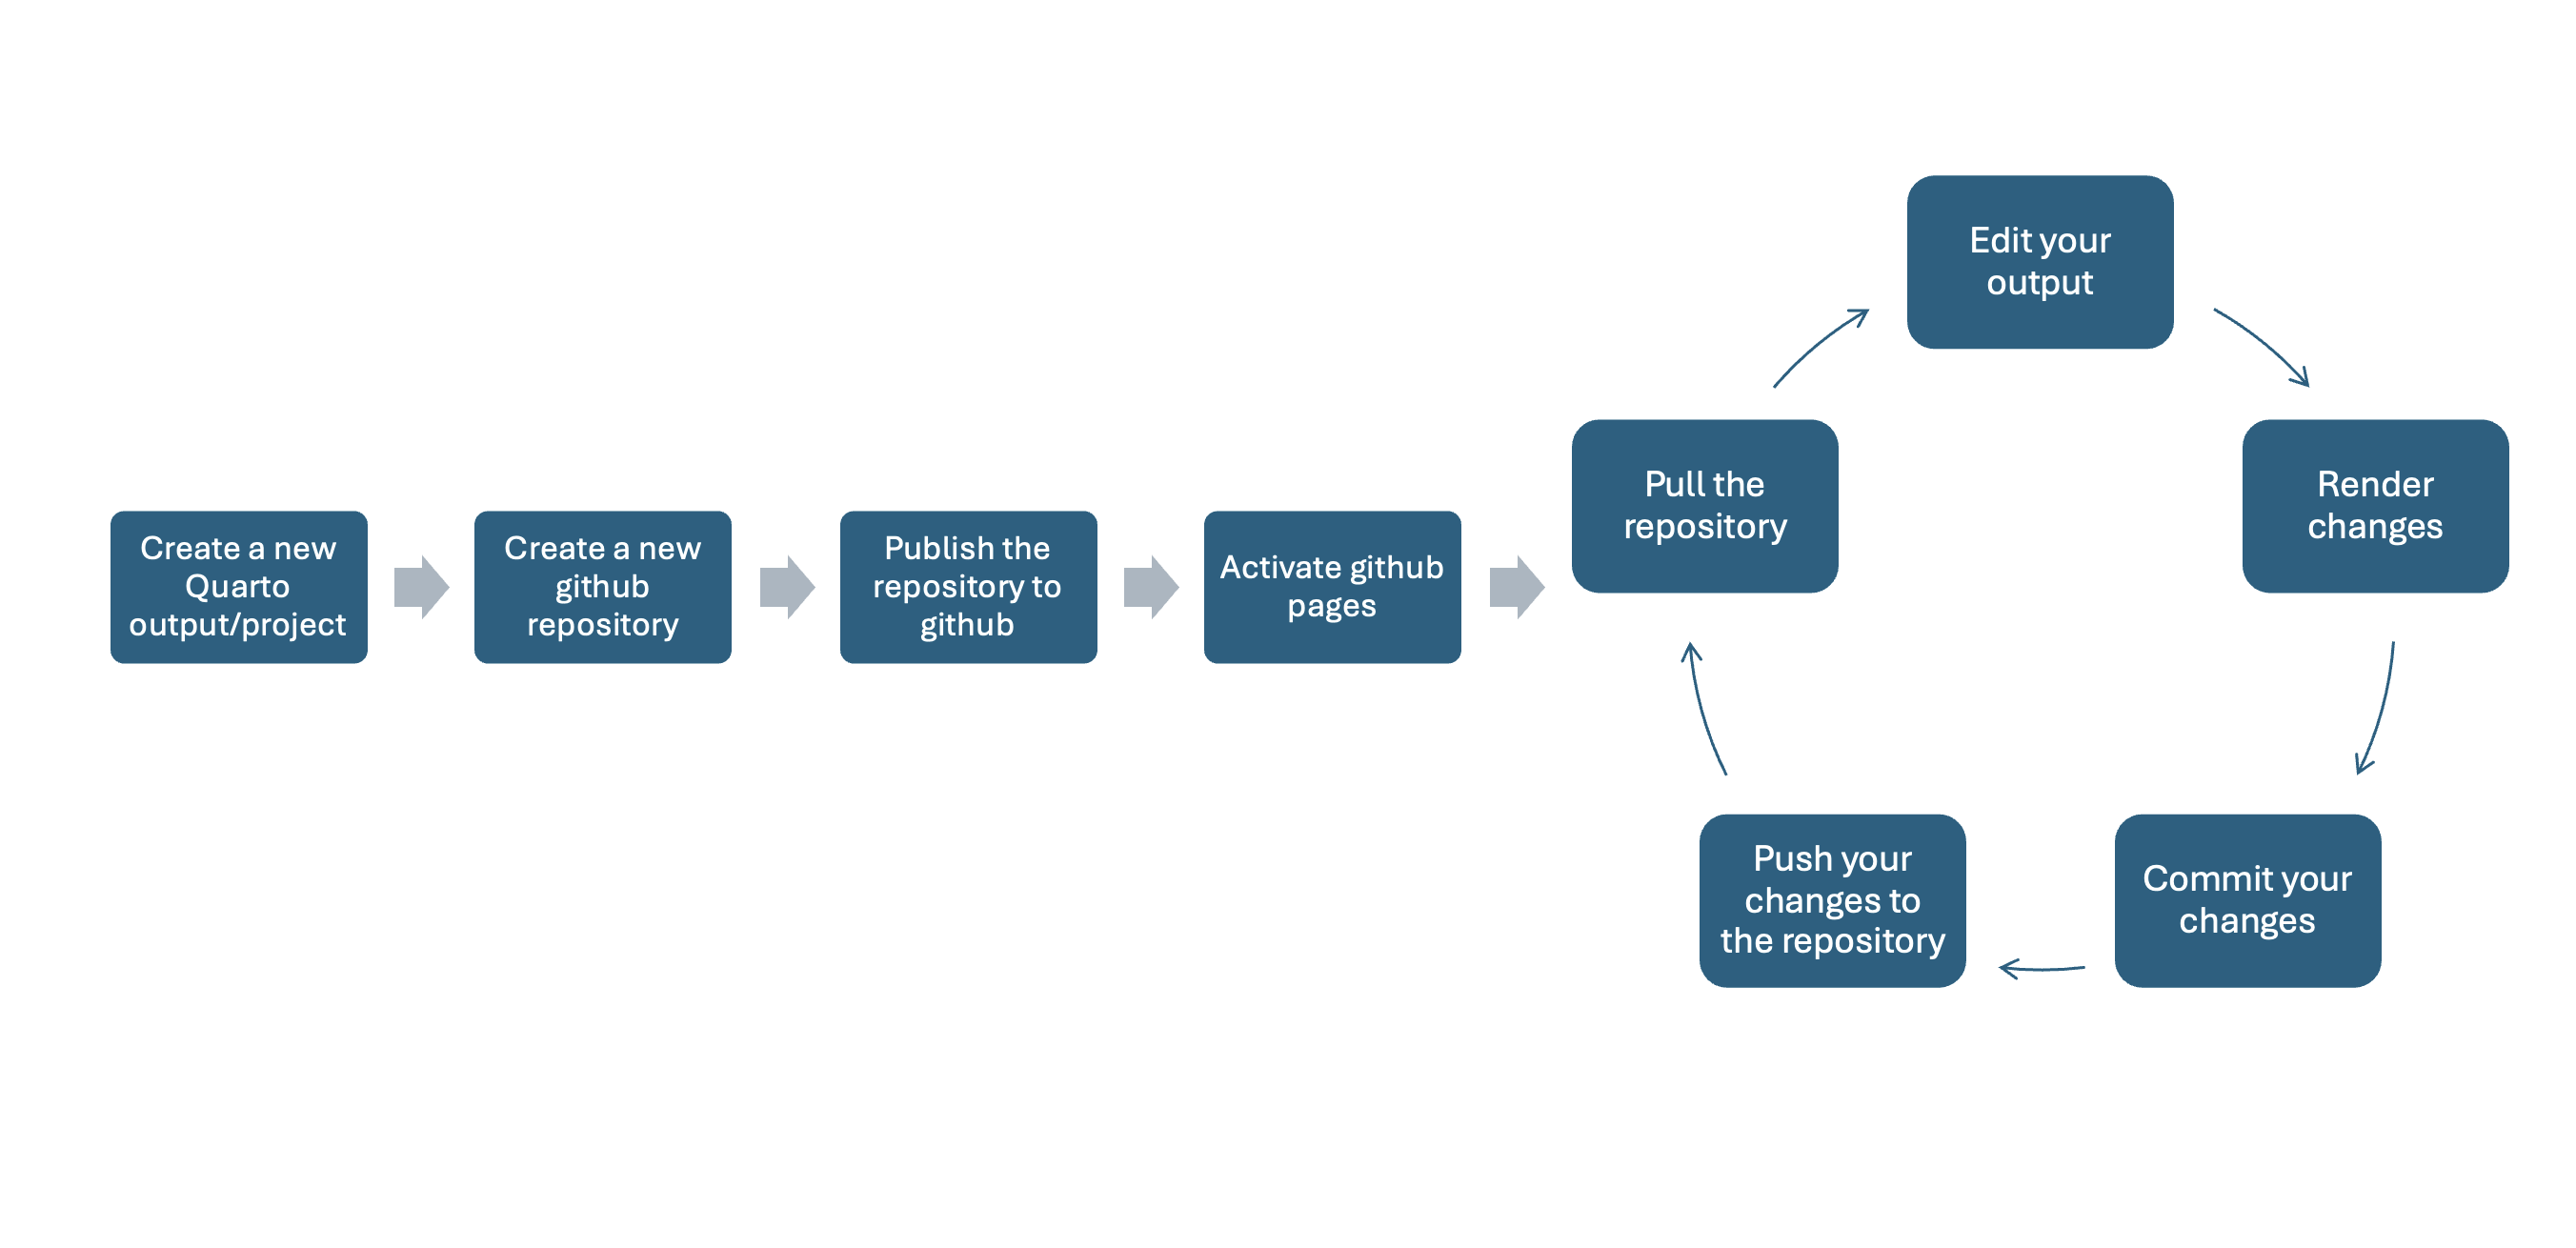
\includegraphics[width=9.01in,height=\textheight]{images/workflow.png}

}

\caption{\label{fig-img-workflow}A flowchart showing the creation and
editing process behind a Quarto output and sharing it using github
pages.}

\end{figure}%

\subsection{Creating your output}\label{creating-your-output}

\begin{enumerate}
\def\labelenumi{\arabic{enumi}.}
\item
  Create a new project to produce the skeleton of your
  book/presentation/website.
\item
  Edit the basic details of your book, like the title, author(s), and
  description.
\item
  Create a new github repository for your output.
\item
  Publish the initial repository so the code is available on github.
\item
  Activate github pages to render the book online via a URL.
\end{enumerate}

\subsection{Editing your output}\label{editing-your-output}

\begin{enumerate}
\def\labelenumi{\arabic{enumi}.}
\item
  Open the output .Rproj file to start working on the materials in
  RStudio.
\item
  Edit or add chapter files in RStudio, specifying their order in the
  \texttt{\_quarto.yml} file.
\item
  Render individual chapter/section files as you work on them. Render
  \texttt{index.qmd} when you want to update all the chapters, or render
  them one by one to ensure all new changes are available.
\item
  Add commits at key points using git/github to mark milestones with
  useful commit messages.
\item
  When you want the book updating, push the changes to be available on
  github and your book URL after a short delay.
\end{enumerate}

\section{Download R and RStudio}\label{download-r-and-rstudio}

If you are new to R/RStudio, you will need to install both pieces of
software which is \emph{normally} pretty straightforward. You might find
this \href{https://youtu.be/YrEe2TLr3MI?si=oweIE55Ul77ZoZwz}{YouTube
video} useful or the \href{https://psyteachr.github.io/RSetGo/}{RSetGo
guide} we prepared for students in the School of Psychology and
Neuroscience.

If you are a more experienced R/RStudio user, just make sure you update
your version of RStudio as Posit are rapidly developing Quarto. I am
currently using R version 4.4.1 (2024-06-14 ucrt) and RStudio
2024.09.1+394, but the more recent the better.

\subsection{Installing Base R}\label{installing-base-r}

\href{https://cran.rstudio.com/}{Install base R}. Choose the download
link for your operating system (Linux, Mac OS X, or Windows).

If you have a Mac, install the latest release from the newest
\texttt{R-x.x.x.pkg} link (or a legacy version if you have an older
operating system). After you install R, you should also install
\href{http://xquartz.macosforge.org/}{XQuartz} to be able to use some
visualisation packages.

If you are installing the Windows version, choose the
``\href{https://cran.rstudio.com/bin/windows/base/}{base}'' subdirectory
and click on the download link at the top of the page. After you install
R, you should also install
\href{https://cran.rstudio.com/bin/windows/Rtools/}{RTools} and use the
``recommended'' version highlighted near the top of the list.

If you are using Linux, choose your specific operating system and follow
the installation instructions. If you use Linux, you probably do not
need help from me.

\subsection{Installing RStudio}\label{installing-rstudio}

Go to
\href{https://www.rstudio.com/products/rstudio/download/\#download}{rstudio.com}
and download the RStudio Desktop version for your operating system. It
should recognise your operating system and allow you to download via the
blue Download button, but you can look for previous versions if you need
one.

\subsection{\texorpdfstring{(optional) Install the \texttt{booktem} R
package}{(optional) Install the booktem R package}}\label{optional-install-the-booktem-r-package}

For one version of a Quarto book, we have a specialised PsyTeachR book
template for the School of Psychology and Neuroscience which you can
use, but it is contained within a package hosted on Prof.~Lisa
DeBruine's github called \texttt{booktem}. To install the package, run
the following code in the Console of RStudio:

\begin{Shaded}
\begin{Highlighting}[]
\NormalTok{devtools}\SpecialCharTok{::}\FunctionTok{install\_github}\NormalTok{(}\StringTok{"debruine/booktem"}\NormalTok{)}
\end{Highlighting}
\end{Shaded}

If you are new to R/RStudio, you probably have no user packages
installed, so you will get a prompt to allow \texttt{booktem} to install
the other R packages it depends on to work. This might take a few
minutes, so go and enjoy yourself a hot drink.

\begin{tcolorbox}[enhanced jigsaw, colbacktitle=quarto-callout-caution-color!10!white, titlerule=0mm, leftrule=.75mm, title=\textcolor{quarto-callout-caution-color}{\faFire}\hspace{0.5em}{Caution}, breakable, bottomrule=.15mm, opacitybacktitle=0.6, rightrule=.15mm, opacityback=0, arc=.35mm, colframe=quarto-callout-caution-color-frame, toptitle=1mm, bottomtitle=1mm, toprule=.15mm, left=2mm, colback=white, coltitle=black]

One of these messages might say something like ``do you want to compile
packages where there is a binary version'' and give you several options
to select. You will only be able to select 1 if you have Rtools
downloaded on a Windows computer as you need developer tools to do this.
Macs should not need any additional software to compile binary packages.
These binary versions are normally a little more recent, so its useful
to install them if possible.

\end{tcolorbox}

If you are a more experienced R/RStudio user, you might be prompted to
update your R packages that \texttt{booktem} depends on. Obviously use
your judgement if you are in a place to update your packages, but the
book template might not work with older packages.

\section{Download git and github desktop}\label{github_prep}

Potentially the most unfamiliar element of this process will be working
with git and github. If you have not used it before, git is a version
control system which tracks file changes on your computer (like OneDrive
but for code). github is an online system which uses git to host those
changes and make your code available online. There is a graphical user
interface called github desktop which I use and will demonstrate. If you
want to use the command line version of git/github, you probably do not
need me to show you how.

There is an
\href{https://github.com/git-guides/install-git}{installation guide} on
github, but we have access to a fantastic resource developed by our
colleagues in Mathematics and Statistics. They developed an accessible
online course on
\href{https://moodle.gla.ac.uk/course/view.php?id=41115}{Moodle}
introducing staff and students to version control using git and github.
You will need the enrollment code \textbf{git\_psych\_24} to access the
course. If you use it, please consider completing their feedback form on
the Moodle page so they can improve the resource in future.

There are 7 units in total which do not take very long, but for the
purposes of this workshop, I would consider 1 and 2 as
\textbf{essential} for downloading git/github desktop and using it as a
single user to track changes. Reaching this point will be super helpful
for following along in the workshop as the terms will be more familiar
to you like repositories, commits, and pushing changes.

If you have time, completing unit 3 will give you everything you need if
you are only using it on your own. If you plan on writing materials in a
team, units 4 and 5 cover being a group project user, then 6 and 7 for
advanced features.

\begin{tcolorbox}[enhanced jigsaw, colbacktitle=quarto-callout-tip-color!10!white, titlerule=0mm, leftrule=.75mm, title=\textcolor{quarto-callout-tip-color}{\faLightbulb}\hspace{0.5em}{Apply for education membership}, breakable, bottomrule=.15mm, opacitybacktitle=0.6, rightrule=.15mm, opacityback=0, arc=.35mm, colframe=quarto-callout-tip-color-frame, toptitle=1mm, bottomtitle=1mm, toprule=.15mm, left=2mm, colback=white, coltitle=black]

The standard version of github should meet all your needs, but by
working at a university you are eligible to apply for an education
membership. If you are interested you can find out more on the
\href{https://github.com/education/teachers}{github education site} for
teachers. For example, with an education profile, you can get unlimited
private repositories.

\end{tcolorbox}

\section{Finished}\label{finished}

You are ready to make your outputs in the workshop or follow along to
the rest of the book here!

\part{Writing Books}

\chapter{Quarto books}\label{quarto_books}

In this chapter, you will learn how to create and edit the standard
version of a Quarto book. This differs to the specific
\hyperref[psyteachr_book]{PsyTeachR template} we cover in the next
chapter. If you do not want additional features built in like
interactive exercises and a glossary function, you may want a more
streamlined version. The editing and rendering process is exactly the
same, it is just the creation process and additional features which
differ.

\textbf{Intended learning outcomes}

By the end of this chapter, you will be able to:

\begin{itemize}
\item
  Create and edit a standard Quarto book using RStudio.
\item
  Publish your book using github pages.
\end{itemize}

\section{Example book}\label{example-book}

For an example of the standard Quarto version, you can explore this very
book on
\href{https://bartlettje.github.io/dissemination_quarto/}{Dissemination
using Quarto and Github Pages}! If there is a feature you like, you can
see the \href{https://github.com/BartlettJE/dissemination_quarto}{source
code on github} to adapt to your needs.

\section{Creating a Quarto book}\label{creating-a-quarto-book}

If you have not followed the \hyperref[workshop_prep]{preparation
instructions} yet, you need R/RStudio and git/github desktop installed
on your computer. I will be demonstrating how to use github desktop
rather than the command line, as git could easily be it's own workshop.

The first step is thinking about where you want your book folder stored
on your computer for where all the files will live. I have a folder
within \texttt{Documents} called \texttt{git\_repos} where I store all
my git repositories away from OneDrive (see below).

\begin{tcolorbox}[enhanced jigsaw, colbacktitle=quarto-callout-warning-color!10!white, titlerule=0mm, leftrule=.75mm, title=\textcolor{quarto-callout-warning-color}{\faExclamationTriangle}\hspace{0.5em}{Do not create github repositories within OneDrive}, breakable, bottomrule=.15mm, opacitybacktitle=0.6, rightrule=.15mm, opacityback=0, arc=.35mm, colframe=quarto-callout-warning-color-frame, toptitle=1mm, bottomtitle=1mm, toprule=.15mm, left=2mm, colback=white, coltitle=black]

We have not reached the github step yet, but as you think about where
you want your folder for the book, please \textbf{do not} use a folder
within OneDrive. Sometimes it works, but most of the time it causes
chaos as OneDrive is trying to track changes, github is trying to track
changes, which ends in them fighting over file permissions.

\end{tcolorbox}

Once you have decided where your book will live, open RStudio and click
\texttt{File\ \textgreater{}\ New\ Project...\ \textgreater{}\ New\ Directory\ \textgreater{}\ Quarto\ book}.
This will be the process we follow for all the Quarto outputs and you
see there are options for a range of documents like websites and blogs.

You will see a new window asking for you to specify:

\begin{itemize}
\item
  ``Directory name:'' - the name of the folder it will create, so keep
  it short and without spaces.
\item
  ``Create a project in the subdirectory of:'' - click browse to
  navigate to the folder you want your book to live in. Creating the
  book will create a new folder within this directory, so you do not
  need to create a folder for the book yourself.
\end{itemize}

Click ``Create project'' and after a couple of seconds, it will open a
new project window with the template in.

Congratulations, you have a book skeleton to work with!

\section{Tour of the Quarto book
template}\label{tour-of-the-quarto-book-template}

\begin{enumerate}
\def\labelenumi{\arabic{enumi}.}
\tightlist
\item
  \texttt{\_quarto.yml}
\end{enumerate}

We will start by exploring the \texttt{\_quarto.yml} file where you can
edit all the details for your book, like the title, author(s), and the
licence. In Quarto books, this is also how you control the order of
chapters.

\begin{tcolorbox}[enhanced jigsaw, colbacktitle=quarto-callout-note-color!10!white, titlerule=0mm, leftrule=.75mm, title=\textcolor{quarto-callout-note-color}{\faInfo}\hspace{0.5em}{What is a .yml file?}, breakable, bottomrule=.15mm, opacitybacktitle=0.6, rightrule=.15mm, opacityback=0, arc=.35mm, colframe=quarto-callout-note-color-frame, toptitle=1mm, bottomtitle=1mm, toprule=.15mm, left=2mm, colback=white, coltitle=black]

YAML / .yml are configuration files for programs which must follow
specific formatting conventions.

\end{tcolorbox}

Within the .yml file, I will highlight in the workshop key features such
as: project, book, bibliography, csl, and format.

For presenting your book using github pages, edit the \texttt{project}
from the standard first two lines:

\begin{Shaded}
\begin{Highlighting}[]
\NormalTok{project}\SpecialCharTok{:}
\NormalTok{  type}\SpecialCharTok{:}\NormalTok{ book}
\end{Highlighting}
\end{Shaded}

To add a new third line:

\begin{Shaded}
\begin{Highlighting}[]
\NormalTok{project}\SpecialCharTok{:}
\NormalTok{  type}\SpecialCharTok{:}\NormalTok{ book}
\NormalTok{  output}\SpecialCharTok{{-}}\NormalTok{dir}\SpecialCharTok{:}\NormalTok{ docs}
\end{Highlighting}
\end{Shaded}

Be careful, indentation is important in .yml files. We do this as by
default, it will create a folder called \texttt{\_book} where the
rendered .html files will live. For github pages though, it looks for a
folder called \texttt{docs}, so this will streamline things later.

\begin{enumerate}
\def\labelenumi{\arabic{enumi}.}
\setcounter{enumi}{1}
\tightlist
\item
  index.qmd
\end{enumerate}

Index will be the opening page for the link to your book, so this will
typically include an overview of what your book contains, who to contact
for problems/questions etc.

\begin{enumerate}
\def\labelenumi{\arabic{enumi}.}
\setcounter{enumi}{2}
\tightlist
\item
  Chapter files
\end{enumerate}

By default, you get an example index.qmd and a few other example
chapters like intro.qmd, summary.qmd, and references.qmd. The example
chapters demonstrate some features of Quarto but you can delete this
text or create your own files to start writing chapters.

You will need one level 1 header (\texttt{\#\ Chapter\ title}) to start
the file, and that will be the name of your chapter at the top of the
page and in the table of contents.

\begin{tcolorbox}[enhanced jigsaw, colbacktitle=quarto-callout-warning-color!10!white, titlerule=0mm, leftrule=.75mm, title=\textcolor{quarto-callout-warning-color}{\faExclamationTriangle}\hspace{0.5em}{Warning}, breakable, bottomrule=.15mm, opacitybacktitle=0.6, rightrule=.15mm, opacityback=0, arc=.35mm, colframe=quarto-callout-warning-color-frame, toptitle=1mm, bottomtitle=1mm, toprule=.15mm, left=2mm, colback=white, coltitle=black]

Make sure you only use one level 1 header per chapter. If you try and
add multiple within one file, it will think they are separate chapters
and try and split them when it renders, making it look weird.

\end{tcolorbox}

Once you start adding multiple chapters, remember to update the .yml
file for the order you want them in your book.

\begin{tcolorbox}[enhanced jigsaw, colbacktitle=quarto-callout-tip-color!10!white, titlerule=0mm, leftrule=.75mm, title=\textcolor{quarto-callout-tip-color}{\faLightbulb}\hspace{0.5em}{Tip}, breakable, bottomrule=.15mm, opacitybacktitle=0.6, rightrule=.15mm, opacityback=0, arc=.35mm, colframe=quarto-callout-tip-color-frame, toptitle=1mm, bottomtitle=1mm, toprule=.15mm, left=2mm, colback=white, coltitle=black]

Depending on what you want to include in your book and how complicated
it becomes, you might want to separate chapters into different sections.
The indentation can be frustrating, but you can add parts to the
\texttt{book:} section of the .yml like:

\begin{Shaded}
\begin{Highlighting}[]
\NormalTok{book}\SpecialCharTok{:}
\NormalTok{  chapters}\SpecialCharTok{:}
    \SpecialCharTok{{-}}\NormalTok{ index.qmd}
    \SpecialCharTok{{-}}\NormalTok{ workshop\_prep.qmd}
    \SpecialCharTok{{-}}\NormalTok{ part}\SpecialCharTok{:} \StringTok{"Writing Books"}
\NormalTok{      chapters}\SpecialCharTok{:}
        \SpecialCharTok{{-}}\NormalTok{ quarto\_books.qmd}
        \SpecialCharTok{{-}}\NormalTok{ psyteachr\_template.qmd}
\end{Highlighting}
\end{Shaded}

\end{tcolorbox}

\begin{enumerate}
\def\labelenumi{\arabic{enumi}.}
\setcounter{enumi}{3}
\tightlist
\item
  references.bib
\end{enumerate}

In the .yml, you can specify a BibTeX file (.bib) to add formatted
citations and references. The template comes with an example for how a
citation and its reference will look. A .bib file stored information for
referencing like authors, the journal, the DOI etc. The Quarto file will
take this information and present it as a citation. The
\hyperref[quarto_features]{Quarto features chapter} explains how to use
a .bib file to format citations and specify a specific citation style.

\begin{enumerate}
\def\labelenumi{\arabic{enumi}.}
\setcounter{enumi}{4}
\tightlist
\item
  Rendering files
\end{enumerate}

Once you have finished editing or you want to check how it looks, you
need to click Render for Quarto to process the code and turn it into
something pretty. Once you click Render once, you can open it up in the
browser and keep checking as you make edits. When you want it to
rerender, click Reload the page and it will show your new edits.

\begin{tcolorbox}[enhanced jigsaw, colbacktitle=quarto-callout-caution-color!10!white, titlerule=0mm, leftrule=.75mm, title=\textcolor{quarto-callout-caution-color}{\faFire}\hspace{0.5em}{Caution}, breakable, bottomrule=.15mm, opacitybacktitle=0.6, rightrule=.15mm, opacityback=0, arc=.35mm, colframe=quarto-callout-caution-color-frame, toptitle=1mm, bottomtitle=1mm, toprule=.15mm, left=2mm, colback=white, coltitle=black]

If you introduce an error, you will get an error and red box on the
screen to highlight Quarto cannot render the book. If you look in the
Background Jobs tab in the console below, you should get an error
message for the source of the problem if you are unsure what you did
wrong.

After an error, you will need to press Render again rather than just
refreshing the browser.

\end{tcolorbox}

These are the key components to make your book. Until this point, these
edits all exist on your own computer. But now it is time to track your
code using github and make your book accessible online via github pages.

\section{Creating a github
repository}\label{creating-a-github-repository}

Once you have a working barebones version of your book ready to go, it's
time to associate your book folder with a github repository and start
some version control. If you want another resource, you can see the
\href{https://docs.github.com/en/desktop/overview/creating-your-first-repository-using-github-desktop}{github
documentation online}.

In future, you could actually start with this part. You can create a new
folder, create a repository using this new folder, and then specify that
folder when you created a project sub directory to add the book file to.
However, we started by creating the book first, so we need to create a
repository for an existing folder without a git component. When you are
used to the process, you can work out which workflow suits you better.

In the github desktop application, click
\texttt{add\ \textgreater{}\textgreater{}\ Create\ a\ New\ Repository}
and complete the details.

\begin{tcolorbox}[enhanced jigsaw, colbacktitle=quarto-callout-warning-color!10!white, titlerule=0mm, leftrule=.75mm, title=\textcolor{quarto-callout-warning-color}{\faExclamationTriangle}\hspace{0.5em}{Seriously, do not create github repositories within OneDrive}, breakable, bottomrule=.15mm, opacitybacktitle=0.6, rightrule=.15mm, opacityback=0, arc=.35mm, colframe=quarto-callout-warning-color-frame, toptitle=1mm, bottomtitle=1mm, toprule=.15mm, left=2mm, colback=white, coltitle=black]

As a reminder, please \textbf{do not} use a folder within OneDrive for
your github repository.

\end{tcolorbox}

\begin{itemize}
\item
  Name: This will be the name of your repository on github, so call it
  something short but sensible. It makes sense to call this the same as
  your book folder wherever possible.
\item
  Local path: Click Choose\ldots{} and navigate to your book folder. You
  want the path to be the main folder your book lives in.
\end{itemize}

The other fields you can edit later, so click ``Create Repository'' when
you are ready.

Your newly minted repository should be showing as the Current
Repository. This exists on your computer, but it is still not available
online. You need to click Publish repository, and that will push all of
your files to github and be available online.

\section{Navigating github and github
pages}\label{navigating-github-and-github-pages}

Now your files are available online, navigate to your github account and
find your new repository.

I will provide a little overview in the workshop of key things to look
out for and what each tab contains.

If you are only interested in using github to work on a book, the key
tabs are Code and Settings. In Code, you will see all your files you
published. These will all be the same as what you created on your
computer. This is the idea behind version control and storing all your
code/files like OneDrive.

In Settings, this is where you can edit things about your repository. If
you plan on working on your book in a team, you can add collaborators by
adding their github profile. They will then receive an email saying you
have invited them to collaborate on their github repository. After they
accept, they can pull the repository and start working on it too.

\begin{tcolorbox}[enhanced jigsaw, colbacktitle=quarto-callout-warning-color!10!white, titlerule=0mm, leftrule=.75mm, title=\textcolor{quarto-callout-warning-color}{\faExclamationTriangle}\hspace{0.5em}{Warning}, breakable, bottomrule=.15mm, opacitybacktitle=0.6, rightrule=.15mm, opacityback=0, arc=.35mm, colframe=quarto-callout-warning-color-frame, toptitle=1mm, bottomtitle=1mm, toprule=.15mm, left=2mm, colback=white, coltitle=black]

Working collaboratively is one of the main motivations behind git and
github, but it can be tricky if you are unfamiliar with more advanced
features like merging and clashes. Before you start editing the same
repository with someone, I \emph{heavily} recommend completing units 4
and 5 of the \hyperref[github_prep]{version control Moodle course}
provided by Maths and Stats.

\end{tcolorbox}

Click on Settings for the next key section we need to get your book
available online.

\subsection{Publish to github pages}\label{publish-to-github-pages}

In Settings, navigate to Pages within Code and automation. Under Build
and deployment, this will be set to none by default. You must click the
drop down, choose Main and select /docs. You will remember /docs is
where we store all the html versions of the book files, so you are
pointing Github pages here as the source for your book.

When you press Save, this will start building your book. It will not be
available immediately and will take a few minutes. When it is ready, at
the top of the page, it will say ``Your site is live at\ldots{}'' with
your new URL you can click on and open. In the Actions tab, it will also
show as a green tick when it has finished building.

Congratulations! After seeing your rendered book for the first time,
this is the second most satisfying part as you can see everything is
working.

\begin{tcolorbox}[enhanced jigsaw, colbacktitle=quarto-callout-tip-color!10!white, titlerule=0mm, leftrule=.75mm, title=\textcolor{quarto-callout-tip-color}{\faLightbulb}\hspace{0.5em}{Add shortcuts to your book}, breakable, bottomrule=.15mm, opacitybacktitle=0.6, rightrule=.15mm, opacityback=0, arc=.35mm, colframe=quarto-callout-tip-color-frame, toptitle=1mm, bottomtitle=1mm, toprule=.15mm, left=2mm, colback=white, coltitle=black]

Once the site is live, I recommend adding the link to two places. First,
save it as a browser shortcut so you can quickly access it outside of
github. Second, return to the Code tab. Click the cog icon next to Above
on the right side and tick to add your website from github pages. This
will show the URL to your book on the Code tab for easy access from
here.

\end{tcolorbox}

\begin{tcolorbox}[enhanced jigsaw, colbacktitle=quarto-callout-tip-color!10!white, titlerule=0mm, leftrule=.75mm, title=\textcolor{quarto-callout-tip-color}{\faLightbulb}\hspace{0.5em}{Customise the URL}, breakable, bottomrule=.15mm, opacitybacktitle=0.6, rightrule=.15mm, opacityback=0, arc=.35mm, colframe=quarto-callout-tip-color-frame, toptitle=1mm, bottomtitle=1mm, toprule=.15mm, left=2mm, colback=white, coltitle=black]

By default, the URL to your book will be your github username +
.github.io + your repository name. If you want to get fancy, you can add
a custom domain from within Settings and Pages if you have bought one.
That is not something we are covering in this workshop or materials
though.

\end{tcolorbox}

\begin{tcolorbox}[enhanced jigsaw, colbacktitle=quarto-callout-warning-color!10!white, titlerule=0mm, leftrule=.75mm, title=\textcolor{quarto-callout-warning-color}{\faExclamationTriangle}\hspace{0.5em}{Warning}, breakable, bottomrule=.15mm, opacitybacktitle=0.6, rightrule=.15mm, opacityback=0, arc=.35mm, colframe=quarto-callout-warning-color-frame, toptitle=1mm, bottomtitle=1mm, toprule=.15mm, left=2mm, colback=white, coltitle=black]

If you try and push a change that contains an error and your book does
not render, you will get a red cross in Actions saying your book did not
build and you will receive an email warning you about it too. Just go
back to the book files in RStudio and fix any errors you are getting
before you push the updates again.

\end{tcolorbox}

\section{Commiting and pushing
changes}\label{commiting-and-pushing-changes}

At this point, you have everything you need for the book workflow. As
you work on your book, you will go through the workflow of:

\begin{enumerate}
\def\labelenumi{\arabic{enumi}.}
\item
  Open .RProj and edit your book in RStudio, either by editing your past
  progress or adding new files.
\item
  When you hit a milestone you want to record, in github desktop tick
  all file changes or specific files, and add a commit message (and
  longer description if necessary).
\item
  If you are continuing to work on the book, keep editing and
  committing.
\item
  When you are ready to push changes to github and github pages, push
  your commits.
\end{enumerate}

Before we have time to start working on your newly minted books, I will
end on a couple of warnings and tips.

\begin{tcolorbox}[enhanced jigsaw, colbacktitle=quarto-callout-caution-color!10!white, titlerule=0mm, leftrule=.75mm, title=\textcolor{quarto-callout-caution-color}{\faFire}\hspace{0.5em}{Caution}, breakable, bottomrule=.15mm, opacitybacktitle=0.6, rightrule=.15mm, opacityback=0, arc=.35mm, colframe=quarto-callout-caution-color-frame, toptitle=1mm, bottomtitle=1mm, toprule=.15mm, left=2mm, colback=white, coltitle=black]

Remember just committing changes will do nothing to your github
repository and book link. You need to push those committed changes for
them to be available on github and used to build the book in github
pages. Likewise, editing the .qmd files and committing the changes to
github will not change anything without first rendering your
chapter/book. You edit the .qmd files but rendering creates the .html
files that display as a website.

It takes a few minutes to rebuild, so do not worry if you do not
immediately see the changes.

\end{tcolorbox}

\begin{tcolorbox}[enhanced jigsaw, colbacktitle=quarto-callout-tip-color!10!white, titlerule=0mm, leftrule=.75mm, title=\textcolor{quarto-callout-tip-color}{\faLightbulb}\hspace{0.5em}{Reverting changes}, breakable, bottomrule=.15mm, opacitybacktitle=0.6, rightrule=.15mm, opacityback=0, arc=.35mm, colframe=quarto-callout-tip-color-frame, toptitle=1mm, bottomtitle=1mm, toprule=.15mm, left=2mm, colback=white, coltitle=black]

One of the main features I use way too infrequently is reverting changes
when something goes wrong. The idea behind version control is you save
your work at specific milestones, where you can add commit messages that
describe key changes you make. If you make a change that breaks
something since your last commit, you can revert the changes to a
previous version. To do this, go to github desktop, click History, and
you will see all your commit history. Identify the last commit you want
to revert to, right click on it, and select Revert Changes in Commit.

\end{tcolorbox}

\section{Start working on your own
book!}\label{start-working-on-your-own-book}

Start working on your own book in the remaining time we have together.

See the final chapter on \hyperref[quarto_features]{Useful Quarto and
booktem features} for inspiration / example code for the kind of
features you can use.

\chapter{PsyTeachR book template}\label{psyteachr_book}

In this chapter, you will see how to use the PsyTeachR book template
developed by Prof.~Lisa DeBruine. This template is what we use for all
the data skills resources in the School of Psychology and Neuroscience.
This has some nice features compared to the standard Quarto book
template, such as supporting webexercises for interactive questions and
including a glossary.

\textbf{Intended learning outcomes}

By the end of this chapter, you will be able to:

\begin{itemize}
\item
  Create and edit a Quarto book using the PsyTeachR template.
\item
  Publish your book using github pages.
\end{itemize}

\section{Example books}\label{example-books}

For a selection of examples of the PsyTeachR book template, you can
explore:

\begin{itemize}
\item
  The \href{https://psyteachr.github.io/quant-fun-v3/}{Fundamentals of
  Quantitative Analysis} book designed for MSc Psychology conversion
  students. If there is a feature you like, you can see the
  \href{https://github.com/PsyTeachR/quant-fun-v3}{source code on
  github} to adapt to your needs.
\item
  The \href{https://psyteachr.github.io/reprores-v4/}{Data Skills for
  Reproducible Research} book designed for MSc Research Methods of
  Psychological Science and MSc Brain Sciences students. If there is a
  feature you like, you can see the
  \href{https://github.com/PsyTeachR/reprores-v4}{source code on github}
  to adapt to your needs.
\end{itemize}

You can see the whole PsyTeachR suite of resources on
\href{https://psyteachr.github.io/}{our website}.

\section{Creating the book template}\label{creating-the-book-template}

If you have not followed the \hyperref[workshop_prep]{preparation
instructions} yet, you need R/RStudio installed to your computer, the
\texttt{booktem} package installed from Lisa's github, and git/github
desktop installed on your computer. I will be demonstrating how to use
github desktop rather than the command line, as git could easily be it's
own workshop.

The first step is thinking about where you want your book folder stored
on your computer, where all the files will live. I have a folder within
\texttt{Documents} called \texttt{git\_repos} where I store all my git
repositories away from OneDrive (see below). You do not need to create a
folder for the book itself as the function will do that for you, but you
need somewhere for that folder to live.

\begin{tcolorbox}[enhanced jigsaw, colbacktitle=quarto-callout-warning-color!10!white, titlerule=0mm, leftrule=.75mm, title=\textcolor{quarto-callout-warning-color}{\faExclamationTriangle}\hspace{0.5em}{Do not create github repositories within OneDrive}, breakable, bottomrule=.15mm, opacitybacktitle=0.6, rightrule=.15mm, opacityback=0, arc=.35mm, colframe=quarto-callout-warning-color-frame, toptitle=1mm, bottomtitle=1mm, toprule=.15mm, left=2mm, colback=white, coltitle=black]

We have not reached the github step yet, but as you think about where
you want your folder for the book, please \textbf{do not} use a folder
within OneDrive. Sometimes it works, but most of the time it causes
chaos as OneDrive is trying to track changes, github is trying to track
changes, which ends in them fighting over file permissions.

\end{tcolorbox}

Once you have a folder your book can live in, open RStudio and set your
working directory to this folder, for example from the top menu
\texttt{Session\ \textgreater{}\textgreater{}\ set\ working\ directory\ \textgreater{}\textgreater{}\ Choose\ directory}
and navigate to this folder.

Once RStudio knows where you want your working directory, you can create
the book using the following code in the console and editing accordingly
before you run the code. Do not worry though, you can edit all of these
later, but this will create the initial version.

\begin{Shaded}
\begin{Highlighting}[]
\CommentTok{\# We first need to load the booktem library, assuming its installed properly}
\FunctionTok{library}\NormalTok{(booktem)}

\FunctionTok{create\_book}\NormalTok{(}\AttributeTok{path =} \StringTok{"your\_book\_file\_name"}\NormalTok{, }\CommentTok{\# If you set your working directory, you should not need to add the full path}
            \AttributeTok{title =} \StringTok{"My book title"}\NormalTok{, }\CommentTok{\# The main title of your book}
            \AttributeTok{authors =} \FunctionTok{list}\NormalTok{( }\CommentTok{\# You need a new line for any additional author, or delete the author 2 line if you\textquotesingle{}re solo}
              \FunctionTok{c}\NormalTok{(}\StringTok{"Author 1 first name"}\NormalTok{, }\StringTok{"Author 1 last name"}\NormalTok{, }\StringTok{"Author 1 ORCiD"}\NormalTok{),}
              \FunctionTok{c}\NormalTok{(}\StringTok{"Author 2 first name"}\NormalTok{, }\StringTok{"Author 2 last name"}\NormalTok{, }\StringTok{"Author 2 ORCiD"}\NormalTok{))}
\NormalTok{            )}
\end{Highlighting}
\end{Shaded}

Once you press run, you should get a bunch of progress messages from
\texttt{Setting\ up\ project...}. Once it's finished, your book will
open in a new session and you will see the rendered version appear in
your default internet browser.

Congratulations, you have a book skeleton to work with!

\section{Tour of the Quarto book
template}\label{tour-of-the-quarto-book-template-1}

\begin{enumerate}
\def\labelenumi{\arabic{enumi}.}
\tightlist
\item
  \texttt{\_quarto.yml}
\end{enumerate}

We will start by exploring the \texttt{\_quarto.yml} file where you can
edit all the details for your book, like the title, description,
author(s), and the licence. In Quarto books, this is also how you
control the order of chapters.

\begin{tcolorbox}[enhanced jigsaw, colbacktitle=quarto-callout-note-color!10!white, titlerule=0mm, leftrule=.75mm, title=\textcolor{quarto-callout-note-color}{\faInfo}\hspace{0.5em}{What is a .yml file?}, breakable, bottomrule=.15mm, opacitybacktitle=0.6, rightrule=.15mm, opacityback=0, arc=.35mm, colframe=quarto-callout-note-color-frame, toptitle=1mm, bottomtitle=1mm, toprule=.15mm, left=2mm, colback=white, coltitle=black]

YAML / .yml are configuration files for programs which must follow
specific formatting conventions.

\end{tcolorbox}

Within the .yml file, I will highlight key features in: project, book,
bibliography, csl, and format.

\begin{enumerate}
\def\labelenumi{\arabic{enumi}.}
\setcounter{enumi}{1}
\tightlist
\item
  index.qmd
\end{enumerate}

Index will be the opening page for the link to your book, so this will
typically include an overview of what your book contains, who to contact
for problems/questions etc.

\begin{enumerate}
\def\labelenumi{\arabic{enumi}.}
\setcounter{enumi}{2}
\tightlist
\item
  \texttt{R/} folder
\end{enumerate}

The \texttt{R/} folder is where you can save bits of R code that your
book relies on. There is some code in here that Lisa has worked on to
help with certain functionality, like how the glossary looks.

\begin{enumerate}
\def\labelenumi{\arabic{enumi}.}
\setcounter{enumi}{3}
\tightlist
\item
  \texttt{include/} folder
\end{enumerate}

The \texttt{include/} folder is a similar idea to \texttt{R/}. It has a
bunch of files the book uses for formatting and any chapters would be
able to access stuff here. For example, a .bib file for your references
and a .csl file for the style of your references.

\begin{enumerate}
\def\labelenumi{\arabic{enumi}.}
\setcounter{enumi}{4}
\tightlist
\item
  \texttt{docs/} folder
\end{enumerate}

The \texttt{docs/} folder is where the rendered .html versions of your
book will update to. The process behind creating books in Quarto is
writing them in Markdown, then Markdown is converted to .html. When we
add the book to github pages, this is the folder you point it to as the
source for how it appears as a webpage.

\begin{enumerate}
\def\labelenumi{\arabic{enumi}.}
\setcounter{enumi}{5}
\tightlist
\item
  Licence
\end{enumerate}

By default, \texttt{booktem} gives the books a CC-BY-SA-4.0 licence.
This is a Creative Commons licence which states people can adapt your
materials but they must provide you with credit. You can learn more
about different types of \href{https://creativecommons.org/}{Creative
Commons licences online}. If you want to state a different licence
depending on your materials, you can update the text in the Licence file
and in the .yml.

\begin{enumerate}
\def\labelenumi{\arabic{enumi}.}
\setcounter{enumi}{6}
\tightlist
\item
  Chapter files
\end{enumerate}

By default, you get an example index.qmd and one chapter .qmd for an
example. The example chapter has a bunch of advice on what to edit and
features like I will demonstrate, but you can delete this text or create
your own files to start writing chapters.

You will need one level 1 header (\texttt{\#\ Chapter\ title}) to start
the file, and that will be the name of your chapter at the top of the
page and in the table of contents.

\begin{tcolorbox}[enhanced jigsaw, colbacktitle=quarto-callout-warning-color!10!white, titlerule=0mm, leftrule=.75mm, title=\textcolor{quarto-callout-warning-color}{\faExclamationTriangle}\hspace{0.5em}{Warning}, breakable, bottomrule=.15mm, opacitybacktitle=0.6, rightrule=.15mm, opacityback=0, arc=.35mm, colframe=quarto-callout-warning-color-frame, toptitle=1mm, bottomtitle=1mm, toprule=.15mm, left=2mm, colback=white, coltitle=black]

Make sure you only use one level 1 header per chapter. If you try and
add multiple within one file, it will think they are separate chapters
and try and split them when it renders, making it look weird.

\end{tcolorbox}

Once you start adding multiple chapters, remember to update the .yml
file for the order you want them in your book.

\begin{tcolorbox}[enhanced jigsaw, colbacktitle=quarto-callout-tip-color!10!white, titlerule=0mm, leftrule=.75mm, title=\textcolor{quarto-callout-tip-color}{\faLightbulb}\hspace{0.5em}{Tip}, breakable, bottomrule=.15mm, opacitybacktitle=0.6, rightrule=.15mm, opacityback=0, arc=.35mm, colframe=quarto-callout-tip-color-frame, toptitle=1mm, bottomtitle=1mm, toprule=.15mm, left=2mm, colback=white, coltitle=black]

If you are converting a previous book to the new template, there is a
handy little function \texttt{rmd2qmd}. This copies .Rmd files and
renames them to .qmd. The function looks like this

\begin{Shaded}
\begin{Highlighting}[]
\FunctionTok{rmd2qmd}\NormalTok{(}\AttributeTok{from\_path =} \StringTok{""}\NormalTok{,  }\CommentTok{\# file path where your .Rmd files are}
        \AttributeTok{to\_path =} \StringTok{""}\NormalTok{) }\CommentTok{\# file path where you want your new .qmd files to go}
\end{Highlighting}
\end{Shaded}

where you specify a file path to access the old .Rmd files and a file
path to where you want the new .qmd files saving. Keep your working
directory in mind as you will probably be starting from your book folder
at this point. I usually save my old .Rmd files in a folder within the
new book directory, then save the new .qmd files to the new book main
directory.

\end{tcolorbox}

\begin{enumerate}
\def\labelenumi{\arabic{enumi}.}
\setcounter{enumi}{7}
\tightlist
\item
  Rendering files
\end{enumerate}

Once you have finished editing or you want to check how it looks, you
need to click Render for Quarto to process the code and turn it into
something pretty. Once you click Render once, you can open it up in the
browser and keep checking as you make edits. When you want it to
rerender, click Reload the page and it will show your new edits.

\begin{tcolorbox}[enhanced jigsaw, colbacktitle=quarto-callout-tip-color!10!white, titlerule=0mm, leftrule=.75mm, title=\textcolor{quarto-callout-tip-color}{\faLightbulb}\hspace{0.5em}{Tip}, breakable, bottomrule=.15mm, opacitybacktitle=0.6, rightrule=.15mm, opacityback=0, arc=.35mm, colframe=quarto-callout-tip-color-frame, toptitle=1mm, bottomtitle=1mm, toprule=.15mm, left=2mm, colback=white, coltitle=black]

The single best part of Quarto and the new book template is you can keep
rendering and checking what your work looks like in the flesh.
Previously, you had to render the whole book to check how it rendered,
but now you can keep updating the browser to see what your changes look
like.

\end{tcolorbox}

\begin{tcolorbox}[enhanced jigsaw, colbacktitle=quarto-callout-caution-color!10!white, titlerule=0mm, leftrule=.75mm, title=\textcolor{quarto-callout-caution-color}{\faFire}\hspace{0.5em}{Caution}, breakable, bottomrule=.15mm, opacitybacktitle=0.6, rightrule=.15mm, opacityback=0, arc=.35mm, colframe=quarto-callout-caution-color-frame, toptitle=1mm, bottomtitle=1mm, toprule=.15mm, left=2mm, colback=white, coltitle=black]

If you introduce an error, you will get an error and red box on the
screen to highlight Quarto cannot render the book. If you look in the
Background Jobs tab in the console below, you should get an error
message for the source of the problem if you are unsure what you did
wrong.

After an error, you will need to press Render again rather than just
refreshing the browser.

\end{tcolorbox}

These are the key components to make your book. Until this point, these
edits all exist on your own computer. But now it is time to track your
code using github and make your book accessible online via github pages.

\section{Creating a github
repository}\label{creating-a-github-repository-1}

Once you have a working barebones version of your book ready to go, it's
time to associate your book folder with a github repository and start
some version control. If you want another resource, you can see the
\href{https://docs.github.com/en/desktop/overview/creating-your-first-repository-using-github-desktop}{github
documentation online}.

In future, you could actually start with this part. You can create a new
folder, create a repository using this new folder, and then use the
\texttt{create\_book()} function to add the book file to. However, we
started by creating the book first, so we need to create a repository
for an existing folder without a git component.

In the github desktop application, click
\texttt{add\ \textgreater{}\textgreater{}\ Create\ a\ New\ Repository}
and complete the details.

\begin{tcolorbox}[enhanced jigsaw, colbacktitle=quarto-callout-warning-color!10!white, titlerule=0mm, leftrule=.75mm, title=\textcolor{quarto-callout-warning-color}{\faExclamationTriangle}\hspace{0.5em}{Seriously, do not create github repositories within OneDrive}, breakable, bottomrule=.15mm, opacitybacktitle=0.6, rightrule=.15mm, opacityback=0, arc=.35mm, colframe=quarto-callout-warning-color-frame, toptitle=1mm, bottomtitle=1mm, toprule=.15mm, left=2mm, colback=white, coltitle=black]

As a reminder, please \textbf{do not} use a folder within OneDrive for
your github repository.

\end{tcolorbox}

\begin{itemize}
\item
  Name: This will be the name of your repository on github, so call it
  something short but sensible.
\item
  Local path: Click Choose\ldots{} and navigate to your book folder. You
  want the path to be the main folder your book lives in.
\end{itemize}

The other fields you can edit later, so click Create Repository when you
are ready.

Your newly minted repository should be showing as the Current
Repository. This exists on your computer, but it is still not available
online. You need to click Publish repository, and that will push all of
your files to github and be available online.

\section{Navigating github and github
pages}\label{navigating-github-and-github-pages-1}

Now your files are available online, navigate to your github account and
find your new repository.

I will provide a little overview in the workshop of key things to look
out for and what each tab contains.

If you are only interested in using github to work on a book, the key
tabs are Code and Settings. In Code, you will see all your files you
published. These will all be the same as what you created on your
computer. This is the idea behind version control and storing all your
code/files like OneDrive.

In Settings, this is where you can edit things about your repository. If
you plan on working on your book in a team, you can add collaborators by
adding their github profile. They will then receive an email saying you
have invited them to collaborate on their github repository. After they
accept, they can pull the repository and start working on it too.

\begin{tcolorbox}[enhanced jigsaw, colbacktitle=quarto-callout-warning-color!10!white, titlerule=0mm, leftrule=.75mm, title=\textcolor{quarto-callout-warning-color}{\faExclamationTriangle}\hspace{0.5em}{Warning}, breakable, bottomrule=.15mm, opacitybacktitle=0.6, rightrule=.15mm, opacityback=0, arc=.35mm, colframe=quarto-callout-warning-color-frame, toptitle=1mm, bottomtitle=1mm, toprule=.15mm, left=2mm, colback=white, coltitle=black]

Working collaboratively is one of the main motivations behind git and
github, but it can be tricky if you are unfamiliar with more advanced
features like merging and clashes. Before you start editing the same
repository with someone, I \emph{heavily} recommend completing units 4
and 5 of the \hyperref[github_prep]{version control Moodle course}
provided by Maths and Stats.

\end{tcolorbox}

Within Settings is the key section we need to get your book available
online.

\subsection{Publish to github pages}\label{publish-to-github-pages-1}

In Settings, navigate to Pages within Code and automation. Under Build
and deployment, this will be set to none by default. You must click the
drop down, choose Main and select /docs. You will remember /docs is
where we store all the html versions of the book files, so you are
pointing Github pages here as the source for your book.

When you press Save, this will start building your book. It will not be
available immediately and will take a few minutes. When it is ready, at
the top of the page, it will say ``Your site is live at\ldots{}'' with
your new URL you can click on and open. In the Actions tab, it will also
show as a green tick when it has finished building.

Congratulations! After seeing your rendered book for the first time,
this is the second most satisfying part as you can see everything is
working.

\begin{tcolorbox}[enhanced jigsaw, colbacktitle=quarto-callout-tip-color!10!white, titlerule=0mm, leftrule=.75mm, title=\textcolor{quarto-callout-tip-color}{\faLightbulb}\hspace{0.5em}{Add shortcuts to your book}, breakable, bottomrule=.15mm, opacitybacktitle=0.6, rightrule=.15mm, opacityback=0, arc=.35mm, colframe=quarto-callout-tip-color-frame, toptitle=1mm, bottomtitle=1mm, toprule=.15mm, left=2mm, colback=white, coltitle=black]

Once the site is live, I recommend adding the link to two places. First,
save it as a browser shortcut so you can quickly access it outside of
github. Second, return to the Code tab. Click the cog icon next to Above
on the right side and tick to add your website from github pages. This
will show the URL to your book on the Code tab for easy access from
here.

\end{tcolorbox}

\begin{tcolorbox}[enhanced jigsaw, colbacktitle=quarto-callout-tip-color!10!white, titlerule=0mm, leftrule=.75mm, title=\textcolor{quarto-callout-tip-color}{\faLightbulb}\hspace{0.5em}{Customise the URL}, breakable, bottomrule=.15mm, opacitybacktitle=0.6, rightrule=.15mm, opacityback=0, arc=.35mm, colframe=quarto-callout-tip-color-frame, toptitle=1mm, bottomtitle=1mm, toprule=.15mm, left=2mm, colback=white, coltitle=black]

By default, the URL to your book will be your github username +
.github.io + your repository name. If you want to get fancy, you can add
a custom domain from within Settings and Pages if you have bought one.

\end{tcolorbox}

\begin{tcolorbox}[enhanced jigsaw, colbacktitle=quarto-callout-warning-color!10!white, titlerule=0mm, leftrule=.75mm, title=\textcolor{quarto-callout-warning-color}{\faExclamationTriangle}\hspace{0.5em}{Warning}, breakable, bottomrule=.15mm, opacitybacktitle=0.6, rightrule=.15mm, opacityback=0, arc=.35mm, colframe=quarto-callout-warning-color-frame, toptitle=1mm, bottomtitle=1mm, toprule=.15mm, left=2mm, colback=white, coltitle=black]

If you try and push a change that contains an error and your book does
not render, you will get a red cross in Actions saying your book did not
build and you will receive an email warning you about it too. Just go
back to the book files in RStudio and fix any errors you are getting
before you push the updates again.

\end{tcolorbox}

\section{Commiting and pushing
changes}\label{commiting-and-pushing-changes-1}

At this point, you have everything you need for the book workflow. As
you work on your book, you will go through the workflow of:

\begin{enumerate}
\def\labelenumi{\arabic{enumi}.}
\item
  Open .RProj and edit your book in RStudio, either by editing your past
  progress or adding new files.
\item
  When you hit a milestone you want to record, in github desktop tick
  all file changes or specific files, and add a commit message (and
  longer description if necessary).
\item
  If you are continuing to work on the book, keeping editing and
  committing.
\item
  When you are ready to push changes to github and github pages, push
  your commits.
\end{enumerate}

Before we have time to start working on your newly minted books, I will
end on a couple of warnings and tips.

\begin{tcolorbox}[enhanced jigsaw, colbacktitle=quarto-callout-caution-color!10!white, titlerule=0mm, leftrule=.75mm, title=\textcolor{quarto-callout-caution-color}{\faFire}\hspace{0.5em}{Caution}, breakable, bottomrule=.15mm, opacitybacktitle=0.6, rightrule=.15mm, opacityback=0, arc=.35mm, colframe=quarto-callout-caution-color-frame, toptitle=1mm, bottomtitle=1mm, toprule=.15mm, left=2mm, colback=white, coltitle=black]

Remember just committing changes will do nothing to your github
repository and book link. You need to push those committed changes for
them to be available on github and used to build the book in github
pages. It takes a few minutes to rebuild, so do not worry if you do not
immediately see the changes.

\end{tcolorbox}

\begin{tcolorbox}[enhanced jigsaw, colbacktitle=quarto-callout-tip-color!10!white, titlerule=0mm, leftrule=.75mm, title=\textcolor{quarto-callout-tip-color}{\faLightbulb}\hspace{0.5em}{Reverting changes}, breakable, bottomrule=.15mm, opacitybacktitle=0.6, rightrule=.15mm, opacityback=0, arc=.35mm, colframe=quarto-callout-tip-color-frame, toptitle=1mm, bottomtitle=1mm, toprule=.15mm, left=2mm, colback=white, coltitle=black]

One of the main features I use way too infrequently is reverting changes
when something goes wrong. The idea behind version control is you save
your work at specific milestones, where you can add commit messages that
describe key changes you make. If you make a change that breaks
something since your last commit, you can revert the changes to a
previous version. To do this, go to github desktop, click History, and
you will see all your commit history. Identify the last commit you want
to revert to, right click on it, and select Revert Changes in Commit.

\end{tcolorbox}

\section{Start working on your own
book!}\label{start-working-on-your-own-book-1}

Start working on your own book in the remaining time we have together.

See the next chapter on \hyperref[quarto_features]{Quarto features and
book conventions} for inspiration / example code for the kind of
features you can use.

Do not forget to make your own hex sticker for extra panache!

\part{Sharing Presentations}

\chapter{Reproducible presentations}\label{quarto_presentations}

In this chapter, you will see how to use the PsyTeachR book template
developed by Prof.~Lisa DeBruine. This template is what we use for all
the data skills resources in the School of Psychology and Neuroscience.
This has some nice features compared to the standard Quarto book
template, such as supporting webexercises for interactive questions and
including a glossary.

\section{Example presentation}\label{example-presentation}

For an example of creating Quarto presentations, you can explore a
\href{https://github.com/BartlettJE/papaja_demo}{papaja demonstration} I
presented for the research centre I am affilated with. If there is a
feature you like, you can see the
\href{https://github.com/BartlettJE/papaja_demo}{source code on github}
to adapt to your needs.

\section{Creating the book template}\label{creating-the-book-template-1}

If you have not followed the \hyperref[workshop_prep]{preparation
instructions} yet, you need R/RStudio installed to your computer, the
\texttt{booktem} package installed from Lisa's github, and git/github
desktop installed on your computer. I will be demonstrating how to use
github desktop rather than the command line, as git could easily be it's
own workshop.

The first step is thinking about where you want your book folder stored
on your computer, where all the files will live. I have a folder within
\texttt{Documents} called \texttt{git\_repos} where I store all my git
repositories away from OneDrive (see below). You do not need to create a
folder for the book itself as the function will do that for you, but you
need somewhere for that folder to live.

\begin{tcolorbox}[enhanced jigsaw, colbacktitle=quarto-callout-warning-color!10!white, titlerule=0mm, leftrule=.75mm, title=\textcolor{quarto-callout-warning-color}{\faExclamationTriangle}\hspace{0.5em}{Do not create github repositories within OneDrive}, breakable, bottomrule=.15mm, opacitybacktitle=0.6, rightrule=.15mm, opacityback=0, arc=.35mm, colframe=quarto-callout-warning-color-frame, toptitle=1mm, bottomtitle=1mm, toprule=.15mm, left=2mm, colback=white, coltitle=black]

We have not reached the github step yet, but as you think about where
you want your folder for the book, please \textbf{do not} use a folder
within OneDrive. Sometimes it works, but most of the time it causes
chaos as OneDrive is trying to track changes, github is trying to track
changes, which ends in them fighting over file permissions.

\end{tcolorbox}

Once you have a folder your book can live in, open RStudio and set your
working directory to this folder, for example from the top menu
\texttt{Session\ \textgreater{}\textgreater{}\ set\ working\ directory\ \textgreater{}\textgreater{}\ Choose\ directory}
and navigate to this folder.

Once RStudio knows where you want your working directory, you can create
the book using the following code in the console and editing accordingly
before you run the code. Do not worry though, you can edit all of these
later, but this will create the initial version.

\begin{Shaded}
\begin{Highlighting}[]
\CommentTok{\# We first need to load the booktem library, assuming its installed properly}
\FunctionTok{library}\NormalTok{(booktem)}

\FunctionTok{create\_book}\NormalTok{(}\AttributeTok{path =} \StringTok{"your\_book\_file\_name"}\NormalTok{, }\CommentTok{\# If you set your working directory, you should not need to add the full path}
            \AttributeTok{title =} \StringTok{"My book title"}\NormalTok{, }\CommentTok{\# The main title of your book}
            \AttributeTok{authors =} \FunctionTok{list}\NormalTok{( }\CommentTok{\# You need a new line for any additional author, or delete the author 2 line if you\textquotesingle{}re solo}
              \FunctionTok{c}\NormalTok{(}\StringTok{"Author 1 first name"}\NormalTok{, }\StringTok{"Author 1 last name"}\NormalTok{, }\StringTok{"Author 1 ORCiD"}\NormalTok{),}
              \FunctionTok{c}\NormalTok{(}\StringTok{"Author 2 first name"}\NormalTok{, }\StringTok{"Author 2 last name"}\NormalTok{, }\StringTok{"Author 2 ORCiD"}\NormalTok{))}
\NormalTok{            )}
\end{Highlighting}
\end{Shaded}

Once you press run, you should get a bunch of progress messages from
\texttt{Setting\ up\ project...}. Once it's finished, your book will
open in a new session and you will see the rendered version appear in
your default internet browser.

Congratulations, you have a book skeleton to work with!

\section{Tour of the Quarto book
template}\label{tour-of-the-quarto-book-template-2}

\begin{enumerate}
\def\labelenumi{\arabic{enumi}.}
\tightlist
\item
  \texttt{\_quarto.yml}
\end{enumerate}

We will start by exploring the \texttt{\_quarto.yml} file where you can
edit all the details for your book, like the title, description,
author(s), and the licence. In Quarto books, this is also how you
control the order of chapters.

\begin{tcolorbox}[enhanced jigsaw, colbacktitle=quarto-callout-note-color!10!white, titlerule=0mm, leftrule=.75mm, title=\textcolor{quarto-callout-note-color}{\faInfo}\hspace{0.5em}{What is a .yml file?}, breakable, bottomrule=.15mm, opacitybacktitle=0.6, rightrule=.15mm, opacityback=0, arc=.35mm, colframe=quarto-callout-note-color-frame, toptitle=1mm, bottomtitle=1mm, toprule=.15mm, left=2mm, colback=white, coltitle=black]

YAML / .yml are configuration files for programs which must follow
specific formatting conventions.

\end{tcolorbox}

Within the .yml file, I will highlight key features in: project, book,
bibliography, csl, and format.

\begin{enumerate}
\def\labelenumi{\arabic{enumi}.}
\setcounter{enumi}{1}
\tightlist
\item
  index.qmd
\end{enumerate}

Index will be the opening page for the link to your book, so this will
typically include an overview of what your book contains, who to contact
for problems/questions etc.

\begin{enumerate}
\def\labelenumi{\arabic{enumi}.}
\setcounter{enumi}{2}
\tightlist
\item
  \texttt{R/} folder
\end{enumerate}

The \texttt{R/} folder is where you can save bits of R code that your
book relies on. There is some code in here that Lisa has worked on to
help with certain functionality, like how the glossary looks.

\begin{enumerate}
\def\labelenumi{\arabic{enumi}.}
\setcounter{enumi}{3}
\tightlist
\item
  \texttt{include/} folder
\end{enumerate}

The \texttt{include/} folder is a similar idea to \texttt{R/}. It has a
bunch of files the book uses for formatting and any chapters would be
able to access stuff here. For example, a .bib file for your references
and a .csl file for the style of your references.

\begin{enumerate}
\def\labelenumi{\arabic{enumi}.}
\setcounter{enumi}{4}
\tightlist
\item
  \texttt{docs/} folder
\end{enumerate}

The \texttt{docs/} folder is where the rendered .html versions of your
book will update to. The process behind creating books in Quarto is
writing them in Markdown, then Markdown is converted to .html. When we
add the book to github pages, this is the folder you point it to as the
source for how it appears as a webpage.

\begin{enumerate}
\def\labelenumi{\arabic{enumi}.}
\setcounter{enumi}{5}
\tightlist
\item
  Licence
\end{enumerate}

By default, \texttt{booktem} gives the books a CC-BY-SA-4.0 licence.
This is a Creative Commons licence which states people can adapt your
materials but they must provide you with credit. You can learn more
about different types of \href{https://creativecommons.org/}{Creative
Commons licences online}. If you want to state a different licence
depending on your materials, you can update the text in the Licence file
and in the .yml.

\begin{enumerate}
\def\labelenumi{\arabic{enumi}.}
\setcounter{enumi}{6}
\tightlist
\item
  Chapter files
\end{enumerate}

By default, you get an example index.qmd and one chapter .qmd for an
example. The example chapter has a bunch of advice on what to edit and
features like I will demonstrate, but you can delete this text or create
your own files to start writing chapters.

You will need one level 1 header (\texttt{\#\ Chapter\ title}) to start
the file, and that will be the name of your chapter at the top of the
page and in the table of contents.

\begin{tcolorbox}[enhanced jigsaw, colbacktitle=quarto-callout-warning-color!10!white, titlerule=0mm, leftrule=.75mm, title=\textcolor{quarto-callout-warning-color}{\faExclamationTriangle}\hspace{0.5em}{Warning}, breakable, bottomrule=.15mm, opacitybacktitle=0.6, rightrule=.15mm, opacityback=0, arc=.35mm, colframe=quarto-callout-warning-color-frame, toptitle=1mm, bottomtitle=1mm, toprule=.15mm, left=2mm, colback=white, coltitle=black]

Make sure you only use one level 1 header per chapter. If you try and
add multiple within one file, it will think they are separate chapters
and try and split them when it renders, making it look weird.

\end{tcolorbox}

Once you start adding multiple chapters, remember to update the .yml
file for the order you want them in your book.

\begin{tcolorbox}[enhanced jigsaw, colbacktitle=quarto-callout-tip-color!10!white, titlerule=0mm, leftrule=.75mm, title=\textcolor{quarto-callout-tip-color}{\faLightbulb}\hspace{0.5em}{Tip}, breakable, bottomrule=.15mm, opacitybacktitle=0.6, rightrule=.15mm, opacityback=0, arc=.35mm, colframe=quarto-callout-tip-color-frame, toptitle=1mm, bottomtitle=1mm, toprule=.15mm, left=2mm, colback=white, coltitle=black]

If you are converting a previous book to the new template, there is a
handy little function \texttt{rmd2qmd}. This copies .Rmd files and
renames them to .qmd. The function looks like this

\begin{Shaded}
\begin{Highlighting}[]
\FunctionTok{rmd2qmd}\NormalTok{(}\AttributeTok{from\_path =} \StringTok{""}\NormalTok{,  }\CommentTok{\# file path where your .Rmd files are}
        \AttributeTok{to\_path =} \StringTok{""}\NormalTok{) }\CommentTok{\# file path where you want your new .qmd files to go}
\end{Highlighting}
\end{Shaded}

where you specify a file path to access the old .Rmd files and a file
path to where you want the new .qmd files saving. Keep your working
directory in mind as you will probably be starting from your book folder
at this point. I usually save my old .Rmd files in a folder within the
new book directory, then save the new .qmd files to the new book main
directory.

\end{tcolorbox}

\begin{enumerate}
\def\labelenumi{\arabic{enumi}.}
\setcounter{enumi}{7}
\tightlist
\item
  Rendering files
\end{enumerate}

Once you have finished editing or you want to check how it looks, you
need to click Render for Quarto to process the code and turn it into
something pretty. Once you click Render once, you can open it up in the
browser and keep checking as you make edits. When you want it to
rerender, click Reload the page and it will show your new edits.

\begin{tcolorbox}[enhanced jigsaw, colbacktitle=quarto-callout-tip-color!10!white, titlerule=0mm, leftrule=.75mm, title=\textcolor{quarto-callout-tip-color}{\faLightbulb}\hspace{0.5em}{Tip}, breakable, bottomrule=.15mm, opacitybacktitle=0.6, rightrule=.15mm, opacityback=0, arc=.35mm, colframe=quarto-callout-tip-color-frame, toptitle=1mm, bottomtitle=1mm, toprule=.15mm, left=2mm, colback=white, coltitle=black]

The single best part of Quarto and the new book template is you can keep
rendering and checking what your work looks like in the flesh.
Previously, you had to render the whole book to check how it rendered,
but now you can keep updating the browser to see what your changes look
like.

\end{tcolorbox}

\begin{tcolorbox}[enhanced jigsaw, colbacktitle=quarto-callout-caution-color!10!white, titlerule=0mm, leftrule=.75mm, title=\textcolor{quarto-callout-caution-color}{\faFire}\hspace{0.5em}{Caution}, breakable, bottomrule=.15mm, opacitybacktitle=0.6, rightrule=.15mm, opacityback=0, arc=.35mm, colframe=quarto-callout-caution-color-frame, toptitle=1mm, bottomtitle=1mm, toprule=.15mm, left=2mm, colback=white, coltitle=black]

If you introduce an error, you will get an error and red box on the
screen to highlight Quarto cannot render the book. If you look in the
Background Jobs tab in the console below, you should get an error
message for the source of the problem if you are unsure what you did
wrong.

After an error, you will need to press Render again rather than just
refreshing the browser.

\end{tcolorbox}

These are the key components to make your book. Until this point, these
edits all exist on your own computer. But now it is time to track your
code using github and make your book accessible online via github pages.

\section{Creating a github
repository}\label{creating-a-github-repository-2}

Once you have a working barebones version of your book ready to go, it's
time to associate your book folder with a github repository and start
some version control. If you want another resource, you can see the
\href{https://docs.github.com/en/desktop/overview/creating-your-first-repository-using-github-desktop}{github
documentation online}.

In future, you could actually start with this part. You can create a new
folder, create a repository using this new folder, and then use the
\texttt{create\_book()} function to add the book file to. However, we
started by creating the book first, so we need to create a repository
for an existing folder without a git component.

In the github desktop application, click
\texttt{add\ \textgreater{}\textgreater{}\ Create\ a\ New\ Repository}
and complete the details.

\begin{tcolorbox}[enhanced jigsaw, colbacktitle=quarto-callout-warning-color!10!white, titlerule=0mm, leftrule=.75mm, title=\textcolor{quarto-callout-warning-color}{\faExclamationTriangle}\hspace{0.5em}{Seriously, do not create github repositories within OneDrive}, breakable, bottomrule=.15mm, opacitybacktitle=0.6, rightrule=.15mm, opacityback=0, arc=.35mm, colframe=quarto-callout-warning-color-frame, toptitle=1mm, bottomtitle=1mm, toprule=.15mm, left=2mm, colback=white, coltitle=black]

As a reminder, please \textbf{do not} use a folder within OneDrive for
your github repository.

\end{tcolorbox}

\begin{itemize}
\item
  Name: This will be the name of your repository on github, so call it
  something short but sensible.
\item
  Local path: Click Choose\ldots{} and navigate to your book folder. You
  want the path to be the main folder your book lives in.
\end{itemize}

The other fields you can edit later, so click Create Repository when you
are ready.

Your newly minted repository should be showing as the Current
Repository. This exists on your computer, but it is still not available
online. You need to click Publish repository, and that will push all of
your files to github and be available online.

\section{Navigating github and github
pages}\label{navigating-github-and-github-pages-2}

Now your files are available online, navigate to your github account and
find your new repository.

I will provide a little overview in the workshop of key things to look
out for and what each tab contains.

If you are only interested in using github to work on a book, the key
tabs are Code and Settings. In Code, you will see all your files you
published. These will all be the same as what you created on your
computer. This is the idea behind version control and storing all your
code/files like OneDrive.

In Settings, this is where you can edit things about your repository. If
you plan on working on your book in a team, you can add collaborators by
adding their github profile. They will then receive an email saying you
have invited them to collaborate on their github repository. After they
accept, they can pull the repository and start working on it too.

\begin{tcolorbox}[enhanced jigsaw, colbacktitle=quarto-callout-warning-color!10!white, titlerule=0mm, leftrule=.75mm, title=\textcolor{quarto-callout-warning-color}{\faExclamationTriangle}\hspace{0.5em}{Warning}, breakable, bottomrule=.15mm, opacitybacktitle=0.6, rightrule=.15mm, opacityback=0, arc=.35mm, colframe=quarto-callout-warning-color-frame, toptitle=1mm, bottomtitle=1mm, toprule=.15mm, left=2mm, colback=white, coltitle=black]

Working collaboratively is one of the main motivations behind git and
github, but it can be tricky if you are unfamiliar with more advanced
features like merging and clashes. Before you start editing the same
repository with someone, I \emph{heavily} recommend completing units 4
and 5 of the \hyperref[github_prep]{version control Moodle course}
provided by Maths and Stats.

\end{tcolorbox}

Within Settings is the key section we need to get your book available
online.

\subsection{Publish to github pages}\label{publish-to-github-pages-2}

In Settings, navigate to Pages within Code and automation. Under Build
and deployment, this will be set to none by default. You must click the
drop down, choose Main and select /docs. You will remember /docs is
where we store all the html versions of the book files, so you are
pointing Github pages here as the source for your book.

When you press Save, this will start building your book. It will not be
available immediately and will take a few minutes. When it is ready, at
the top of the page, it will say ``Your site is live at\ldots{}'' with
your new URL you can click on and open. In the Actions tab, it will also
show as a green tick when it has finished building.

Congratulations! After seeing your rendered book for the first time,
this is the second most satisfying part as you can see everything is
working.

\begin{tcolorbox}[enhanced jigsaw, colbacktitle=quarto-callout-tip-color!10!white, titlerule=0mm, leftrule=.75mm, title=\textcolor{quarto-callout-tip-color}{\faLightbulb}\hspace{0.5em}{Add shortcuts to your book}, breakable, bottomrule=.15mm, opacitybacktitle=0.6, rightrule=.15mm, opacityback=0, arc=.35mm, colframe=quarto-callout-tip-color-frame, toptitle=1mm, bottomtitle=1mm, toprule=.15mm, left=2mm, colback=white, coltitle=black]

Once the site is live, I recommend adding the link to two places. First,
save it as a browser shortcut so you can quickly access it outside of
github. Second, return to the Code tab. Click the cog icon next to Above
on the right side and tick to add your website from github pages. This
will show the URL to your book on the Code tab for easy access from
here.

\end{tcolorbox}

\begin{tcolorbox}[enhanced jigsaw, colbacktitle=quarto-callout-tip-color!10!white, titlerule=0mm, leftrule=.75mm, title=\textcolor{quarto-callout-tip-color}{\faLightbulb}\hspace{0.5em}{Customise the URL}, breakable, bottomrule=.15mm, opacitybacktitle=0.6, rightrule=.15mm, opacityback=0, arc=.35mm, colframe=quarto-callout-tip-color-frame, toptitle=1mm, bottomtitle=1mm, toprule=.15mm, left=2mm, colback=white, coltitle=black]

By default, the URL to your book will be your github username +
.github.io + your repository name. If you want to get fancy, you can add
a custom domain from within Settings and Pages if you have bought one.

\end{tcolorbox}

\begin{tcolorbox}[enhanced jigsaw, colbacktitle=quarto-callout-warning-color!10!white, titlerule=0mm, leftrule=.75mm, title=\textcolor{quarto-callout-warning-color}{\faExclamationTriangle}\hspace{0.5em}{Warning}, breakable, bottomrule=.15mm, opacitybacktitle=0.6, rightrule=.15mm, opacityback=0, arc=.35mm, colframe=quarto-callout-warning-color-frame, toptitle=1mm, bottomtitle=1mm, toprule=.15mm, left=2mm, colback=white, coltitle=black]

If you try and push a change that contains an error and your book does
not render, you will get a red cross in Actions saying your book did not
build and you will receive an email warning you about it too. Just go
back to the book files in RStudio and fix any errors you are getting
before you push the updates again.

\end{tcolorbox}

\section{Commiting and pushing
changes}\label{commiting-and-pushing-changes-2}

At this point, you have everything you need for the book workflow. As
you work on your book, you will go through the workflow of:

\begin{enumerate}
\def\labelenumi{\arabic{enumi}.}
\item
  Open .RProj and edit your book in RStudio, either by editing your past
  progress or adding new files.
\item
  When you hit a milestone you want to record, in github desktop tick
  all file changes or specific files, and add a commit message (and
  longer description if necessary).
\item
  If you are continuing to work on the book, keeping editing and
  committing.
\item
  When you are ready to push changes to github and github pages, push
  your commits.
\end{enumerate}

Before we have time to start working on your newly minted books, I will
end on a couple of warnings and tips.

\begin{tcolorbox}[enhanced jigsaw, colbacktitle=quarto-callout-caution-color!10!white, titlerule=0mm, leftrule=.75mm, title=\textcolor{quarto-callout-caution-color}{\faFire}\hspace{0.5em}{Caution}, breakable, bottomrule=.15mm, opacitybacktitle=0.6, rightrule=.15mm, opacityback=0, arc=.35mm, colframe=quarto-callout-caution-color-frame, toptitle=1mm, bottomtitle=1mm, toprule=.15mm, left=2mm, colback=white, coltitle=black]

Remember just committing changes will do nothing to your github
repository and book link. You need to push those committed changes for
them to be available on github and used to build the book in github
pages. It takes a few minutes to rebuild, so do not worry if you do not
immediately see the changes.

\end{tcolorbox}

\begin{tcolorbox}[enhanced jigsaw, colbacktitle=quarto-callout-tip-color!10!white, titlerule=0mm, leftrule=.75mm, title=\textcolor{quarto-callout-tip-color}{\faLightbulb}\hspace{0.5em}{Reverting changes}, breakable, bottomrule=.15mm, opacitybacktitle=0.6, rightrule=.15mm, opacityback=0, arc=.35mm, colframe=quarto-callout-tip-color-frame, toptitle=1mm, bottomtitle=1mm, toprule=.15mm, left=2mm, colback=white, coltitle=black]

One of the main features I use way too infrequently is reverting changes
when something goes wrong. The idea behind version control is you save
your work at specific milestones, where you can add commit messages that
describe key changes you make. If you make a change that breaks
something since your last commit, you can revert the changes to a
previous version. To do this, go to github desktop, click History, and
you will see all your commit history. Identify the last commit you want
to revert to, right click on it, and select Revert Changes in Commit.

\end{tcolorbox}

\section{Start working on your own
book!}\label{start-working-on-your-own-book-2}

Start working on your own book in the remaining time we have together.

See the next chapter on \hyperref[quarto_features]{Quarto features and
book conventions} for inspiration / example code for the kind of
features you can use.

Do not forget to make your own hex sticker for extra panache!

\part{Creating Websites}

\chapter{Websites and blogs}\label{quarto_websites}

In this chapter, you will see how to use the PsyTeachR book template
developed by Prof.~Lisa DeBruine. This template is what we use for all
the data skills resources in the School of Psychology and Neuroscience.
This has some nice features compared to the standard Quarto book
template, such as supporting webexercises for interactive questions and
including a glossary.

\section{Example book}\label{example-book-1}

For an example of the PsyTeachR book template, you can explore the
\href{https://psyteachr.github.io/quant-fun-v3/}{Fundamentals of
Quantitative Analysis} book. If there is a feature you like, you can see
the \href{https://github.com/PsyTeachR/quant-fun-v3}{source code on
github} to adapt to your needs.

\section{Creating the book template}\label{creating-the-book-template-2}

If you have not followed the \hyperref[workshop_prep]{preparation
instructions} yet, you need R/RStudio installed to your computer, the
\texttt{booktem} package installed from Lisa's github, and git/github
desktop installed on your computer. I will be demonstrating how to use
github desktop rather than the command line, as git could easily be it's
own workshop.

The first step is thinking about where you want your book folder stored
on your computer, where all the files will live. I have a folder within
\texttt{Documents} called \texttt{git\_repos} where I store all my git
repositories away from OneDrive (see below). You do not need to create a
folder for the book itself as the function will do that for you, but you
need somewhere for that folder to live.

\begin{tcolorbox}[enhanced jigsaw, colbacktitle=quarto-callout-warning-color!10!white, titlerule=0mm, leftrule=.75mm, title=\textcolor{quarto-callout-warning-color}{\faExclamationTriangle}\hspace{0.5em}{Do not create github repositories within OneDrive}, breakable, bottomrule=.15mm, opacitybacktitle=0.6, rightrule=.15mm, opacityback=0, arc=.35mm, colframe=quarto-callout-warning-color-frame, toptitle=1mm, bottomtitle=1mm, toprule=.15mm, left=2mm, colback=white, coltitle=black]

We have not reached the github step yet, but as you think about where
you want your folder for the book, please \textbf{do not} use a folder
within OneDrive. Sometimes it works, but most of the time it causes
chaos as OneDrive is trying to track changes, github is trying to track
changes, which ends in them fighting over file permissions.

\end{tcolorbox}

Once you have a folder your book can live in, open RStudio and set your
working directory to this folder, for example from the top menu
\texttt{Session\ \textgreater{}\textgreater{}\ set\ working\ directory\ \textgreater{}\textgreater{}\ Choose\ directory}
and navigate to this folder.

Once RStudio knows where you want your working directory, you can create
the book using the following code in the console and editing accordingly
before you run the code. Do not worry though, you can edit all of these
later, but this will create the initial version.

\begin{Shaded}
\begin{Highlighting}[]
\CommentTok{\# We first need to load the booktem library, assuming its installed properly}
\FunctionTok{library}\NormalTok{(booktem)}

\FunctionTok{create\_book}\NormalTok{(}\AttributeTok{path =} \StringTok{"your\_book\_file\_name"}\NormalTok{, }\CommentTok{\# If you set your working directory, you should not need to add the full path}
            \AttributeTok{title =} \StringTok{"My book title"}\NormalTok{, }\CommentTok{\# The main title of your book}
            \AttributeTok{authors =} \FunctionTok{list}\NormalTok{( }\CommentTok{\# You need a new line for any additional author, or delete the author 2 line if you\textquotesingle{}re solo}
              \FunctionTok{c}\NormalTok{(}\StringTok{"Author 1 first name"}\NormalTok{, }\StringTok{"Author 1 last name"}\NormalTok{, }\StringTok{"Author 1 ORCiD"}\NormalTok{),}
              \FunctionTok{c}\NormalTok{(}\StringTok{"Author 2 first name"}\NormalTok{, }\StringTok{"Author 2 last name"}\NormalTok{, }\StringTok{"Author 2 ORCiD"}\NormalTok{))}
\NormalTok{            )}
\end{Highlighting}
\end{Shaded}

Once you press run, you should get a bunch of progress messages from
\texttt{Setting\ up\ project...}. Once it's finished, your book will
open in a new session and you will see the rendered version appear in
your default internet browser.

Congratulations, you have a book skeleton to work with!

\section{Tour of the Quarto book
template}\label{tour-of-the-quarto-book-template-3}

\begin{enumerate}
\def\labelenumi{\arabic{enumi}.}
\tightlist
\item
  \texttt{\_quarto.yml}
\end{enumerate}

We will start by exploring the \texttt{\_quarto.yml} file where you can
edit all the details for your book, like the title, description,
author(s), and the licence. In Quarto books, this is also how you
control the order of chapters.

\begin{tcolorbox}[enhanced jigsaw, colbacktitle=quarto-callout-note-color!10!white, titlerule=0mm, leftrule=.75mm, title=\textcolor{quarto-callout-note-color}{\faInfo}\hspace{0.5em}{What is a .yml file?}, breakable, bottomrule=.15mm, opacitybacktitle=0.6, rightrule=.15mm, opacityback=0, arc=.35mm, colframe=quarto-callout-note-color-frame, toptitle=1mm, bottomtitle=1mm, toprule=.15mm, left=2mm, colback=white, coltitle=black]

YAML / .yml are configuration files for programs which must follow
specific formatting conventions.

\end{tcolorbox}

Within the .yml file, I will highlight key features in: project, book,
bibliography, csl, and format.

\begin{enumerate}
\def\labelenumi{\arabic{enumi}.}
\setcounter{enumi}{1}
\tightlist
\item
  index.qmd
\end{enumerate}

Index will be the opening page for the link to your book, so this will
typically include an overview of what your book contains, who to contact
for problems/questions etc.

\begin{enumerate}
\def\labelenumi{\arabic{enumi}.}
\setcounter{enumi}{2}
\tightlist
\item
  \texttt{R/} folder
\end{enumerate}

The \texttt{R/} folder is where you can save bits of R code that your
book relies on. There is some code in here that Lisa has worked on to
help with certain functionality, like how the glossary looks.

\begin{enumerate}
\def\labelenumi{\arabic{enumi}.}
\setcounter{enumi}{3}
\tightlist
\item
  \texttt{include/} folder
\end{enumerate}

The \texttt{include/} folder is a similar idea to \texttt{R/}. It has a
bunch of files the book uses for formatting and any chapters would be
able to access stuff here. For example, a .bib file for your references
and a .csl file for the style of your references.

\begin{enumerate}
\def\labelenumi{\arabic{enumi}.}
\setcounter{enumi}{4}
\tightlist
\item
  \texttt{docs/} folder
\end{enumerate}

The \texttt{docs/} folder is where the rendered .html versions of your
book will update to. The process behind creating books in Quarto is
writing them in Markdown, then Markdown is converted to .html. When we
add the book to github pages, this is the folder you point it to as the
source for how it appears as a webpage.

\begin{enumerate}
\def\labelenumi{\arabic{enumi}.}
\setcounter{enumi}{5}
\tightlist
\item
  Licence
\end{enumerate}

By default, \texttt{booktem} gives the books a CC-BY-SA-4.0 licence.
This is a Creative Commons licence which states people can adapt your
materials but they must provide you with credit. You can learn more
about different types of \href{https://creativecommons.org/}{Creative
Commons licences online}. If you want to state a different licence
depending on your materials, you can update the text in the Licence file
and in the .yml.

\begin{enumerate}
\def\labelenumi{\arabic{enumi}.}
\setcounter{enumi}{6}
\tightlist
\item
  Chapter files
\end{enumerate}

By default, you get an example index.qmd and one chapter .qmd for an
example. The example chapter has a bunch of advice on what to edit and
features like I will demonstrate, but you can delete this text or create
your own files to start writing chapters.

You will need one level 1 header (\texttt{\#\ Chapter\ title}) to start
the file, and that will be the name of your chapter at the top of the
page and in the table of contents.

\begin{tcolorbox}[enhanced jigsaw, colbacktitle=quarto-callout-warning-color!10!white, titlerule=0mm, leftrule=.75mm, title=\textcolor{quarto-callout-warning-color}{\faExclamationTriangle}\hspace{0.5em}{Warning}, breakable, bottomrule=.15mm, opacitybacktitle=0.6, rightrule=.15mm, opacityback=0, arc=.35mm, colframe=quarto-callout-warning-color-frame, toptitle=1mm, bottomtitle=1mm, toprule=.15mm, left=2mm, colback=white, coltitle=black]

Make sure you only use one level 1 header per chapter. If you try and
add multiple within one file, it will think they are separate chapters
and try and split them when it renders, making it look weird.

\end{tcolorbox}

Once you start adding multiple chapters, remember to update the .yml
file for the order you want them in your book.

\begin{tcolorbox}[enhanced jigsaw, colbacktitle=quarto-callout-tip-color!10!white, titlerule=0mm, leftrule=.75mm, title=\textcolor{quarto-callout-tip-color}{\faLightbulb}\hspace{0.5em}{Tip}, breakable, bottomrule=.15mm, opacitybacktitle=0.6, rightrule=.15mm, opacityback=0, arc=.35mm, colframe=quarto-callout-tip-color-frame, toptitle=1mm, bottomtitle=1mm, toprule=.15mm, left=2mm, colback=white, coltitle=black]

If you are converting a previous book to the new template, there is a
handy little function \texttt{rmd2qmd}. This copies .Rmd files and
renames them to .qmd. The function looks like this

\begin{Shaded}
\begin{Highlighting}[]
\FunctionTok{rmd2qmd}\NormalTok{(}\AttributeTok{from\_path =} \StringTok{""}\NormalTok{,  }\CommentTok{\# file path where your .Rmd files are}
        \AttributeTok{to\_path =} \StringTok{""}\NormalTok{) }\CommentTok{\# file path where you want your new .qmd files to go}
\end{Highlighting}
\end{Shaded}

where you specify a file path to access the old .Rmd files and a file
path to where you want the new .qmd files saving. Keep your working
directory in mind as you will probably be starting from your book folder
at this point. I usually save my old .Rmd files in a folder within the
new book directory, then save the new .qmd files to the new book main
directory.

\end{tcolorbox}

\begin{enumerate}
\def\labelenumi{\arabic{enumi}.}
\setcounter{enumi}{7}
\tightlist
\item
  Rendering files
\end{enumerate}

Once you have finished editing or you want to check how it looks, you
need to click Render for Quarto to process the code and turn it into
something pretty. Once you click Render once, you can open it up in the
browser and keep checking as you make edits. When you want it to
rerender, click Reload the page and it will show your new edits.

\begin{tcolorbox}[enhanced jigsaw, colbacktitle=quarto-callout-tip-color!10!white, titlerule=0mm, leftrule=.75mm, title=\textcolor{quarto-callout-tip-color}{\faLightbulb}\hspace{0.5em}{Tip}, breakable, bottomrule=.15mm, opacitybacktitle=0.6, rightrule=.15mm, opacityback=0, arc=.35mm, colframe=quarto-callout-tip-color-frame, toptitle=1mm, bottomtitle=1mm, toprule=.15mm, left=2mm, colback=white, coltitle=black]

The single best part of Quarto and the new book template is you can keep
rendering and checking what your work looks like in the flesh.
Previously, you had to render the whole book to check how it rendered,
but now you can keep updating the browser to see what your changes look
like.

\end{tcolorbox}

\begin{tcolorbox}[enhanced jigsaw, colbacktitle=quarto-callout-caution-color!10!white, titlerule=0mm, leftrule=.75mm, title=\textcolor{quarto-callout-caution-color}{\faFire}\hspace{0.5em}{Caution}, breakable, bottomrule=.15mm, opacitybacktitle=0.6, rightrule=.15mm, opacityback=0, arc=.35mm, colframe=quarto-callout-caution-color-frame, toptitle=1mm, bottomtitle=1mm, toprule=.15mm, left=2mm, colback=white, coltitle=black]

If you introduce an error, you will get an error and red box on the
screen to highlight Quarto cannot render the book. If you look in the
Background Jobs tab in the console below, you should get an error
message for the source of the problem if you are unsure what you did
wrong.

After an error, you will need to press Render again rather than just
refreshing the browser.

\end{tcolorbox}

These are the key components to make your book. Until this point, these
edits all exist on your own computer. But now it is time to track your
code using github and make your book accessible online via github pages.

\section{Creating a github
repository}\label{creating-a-github-repository-3}

Once you have a working barebones version of your book ready to go, it's
time to associate your book folder with a github repository and start
some version control. If you want another resource, you can see the
\href{https://docs.github.com/en/desktop/overview/creating-your-first-repository-using-github-desktop}{github
documentation online}.

In future, you could actually start with this part. You can create a new
folder, create a repository using this new folder, and then use the
\texttt{create\_book()} function to add the book file to. However, we
started by creating the book first, so we need to create a repository
for an existing folder without a git component.

In the github desktop application, click
\texttt{add\ \textgreater{}\textgreater{}\ Create\ a\ New\ Repository}
and complete the details.

\begin{tcolorbox}[enhanced jigsaw, colbacktitle=quarto-callout-warning-color!10!white, titlerule=0mm, leftrule=.75mm, title=\textcolor{quarto-callout-warning-color}{\faExclamationTriangle}\hspace{0.5em}{Seriously, do not create github repositories within OneDrive}, breakable, bottomrule=.15mm, opacitybacktitle=0.6, rightrule=.15mm, opacityback=0, arc=.35mm, colframe=quarto-callout-warning-color-frame, toptitle=1mm, bottomtitle=1mm, toprule=.15mm, left=2mm, colback=white, coltitle=black]

As a reminder, please \textbf{do not} use a folder within OneDrive for
your github repository.

\end{tcolorbox}

\begin{itemize}
\item
  Name: This will be the name of your repository on github, so call it
  something short but sensible.
\item
  Local path: Click Choose\ldots{} and navigate to your book folder. You
  want the path to be the main folder your book lives in.
\end{itemize}

The other fields you can edit later, so click Create Repository when you
are ready.

Your newly minted repository should be showing as the Current
Repository. This exists on your computer, but it is still not available
online. You need to click Publish repository, and that will push all of
your files to github and be available online.

\section{Navigating github and github
pages}\label{navigating-github-and-github-pages-3}

Now your files are available online, navigate to your github account and
find your new repository.

I will provide a little overview in the workshop of key things to look
out for and what each tab contains.

If you are only interested in using github to work on a book, the key
tabs are Code and Settings. In Code, you will see all your files you
published. These will all be the same as what you created on your
computer. This is the idea behind version control and storing all your
code/files like OneDrive.

In Settings, this is where you can edit things about your repository. If
you plan on working on your book in a team, you can add collaborators by
adding their github profile. They will then receive an email saying you
have invited them to collaborate on their github repository. After they
accept, they can pull the repository and start working on it too.

\begin{tcolorbox}[enhanced jigsaw, colbacktitle=quarto-callout-warning-color!10!white, titlerule=0mm, leftrule=.75mm, title=\textcolor{quarto-callout-warning-color}{\faExclamationTriangle}\hspace{0.5em}{Warning}, breakable, bottomrule=.15mm, opacitybacktitle=0.6, rightrule=.15mm, opacityback=0, arc=.35mm, colframe=quarto-callout-warning-color-frame, toptitle=1mm, bottomtitle=1mm, toprule=.15mm, left=2mm, colback=white, coltitle=black]

Working collaboratively is one of the main motivations behind git and
github, but it can be tricky if you are unfamiliar with more advanced
features like merging and clashes. Before you start editing the same
repository with someone, I \emph{heavily} recommend completing units 4
and 5 of the \hyperref[github_prep]{version control Moodle course}
provided by Maths and Stats.

\end{tcolorbox}

Within Settings is the key section we need to get your book available
online.

\subsection{Publish to github pages}\label{publish-to-github-pages-3}

In Settings, navigate to Pages within Code and automation. Under Build
and deployment, this will be set to none by default. You must click the
drop down, choose Main and select /docs. You will remember /docs is
where we store all the html versions of the book files, so you are
pointing Github pages here as the source for your book.

When you press Save, this will start building your book. It will not be
available immediately and will take a few minutes. When it is ready, at
the top of the page, it will say ``Your site is live at\ldots{}'' with
your new URL you can click on and open. In the Actions tab, it will also
show as a green tick when it has finished building.

Congratulations! After seeing your rendered book for the first time,
this is the second most satisfying part as you can see everything is
working.

\begin{tcolorbox}[enhanced jigsaw, colbacktitle=quarto-callout-tip-color!10!white, titlerule=0mm, leftrule=.75mm, title=\textcolor{quarto-callout-tip-color}{\faLightbulb}\hspace{0.5em}{Add shortcuts to your book}, breakable, bottomrule=.15mm, opacitybacktitle=0.6, rightrule=.15mm, opacityback=0, arc=.35mm, colframe=quarto-callout-tip-color-frame, toptitle=1mm, bottomtitle=1mm, toprule=.15mm, left=2mm, colback=white, coltitle=black]

Once the site is live, I recommend adding the link to two places. First,
save it as a browser shortcut so you can quickly access it outside of
github. Second, return to the Code tab. Click the cog icon next to Above
on the right side and tick to add your website from github pages. This
will show the URL to your book on the Code tab for easy access from
here.

\end{tcolorbox}

\begin{tcolorbox}[enhanced jigsaw, colbacktitle=quarto-callout-tip-color!10!white, titlerule=0mm, leftrule=.75mm, title=\textcolor{quarto-callout-tip-color}{\faLightbulb}\hspace{0.5em}{Customise the URL}, breakable, bottomrule=.15mm, opacitybacktitle=0.6, rightrule=.15mm, opacityback=0, arc=.35mm, colframe=quarto-callout-tip-color-frame, toptitle=1mm, bottomtitle=1mm, toprule=.15mm, left=2mm, colback=white, coltitle=black]

By default, the URL to your book will be your github username +
.github.io + your repository name. If you want to get fancy, you can add
a custom domain from within Settings and Pages if you have bought one.

\end{tcolorbox}

\begin{tcolorbox}[enhanced jigsaw, colbacktitle=quarto-callout-warning-color!10!white, titlerule=0mm, leftrule=.75mm, title=\textcolor{quarto-callout-warning-color}{\faExclamationTriangle}\hspace{0.5em}{Warning}, breakable, bottomrule=.15mm, opacitybacktitle=0.6, rightrule=.15mm, opacityback=0, arc=.35mm, colframe=quarto-callout-warning-color-frame, toptitle=1mm, bottomtitle=1mm, toprule=.15mm, left=2mm, colback=white, coltitle=black]

If you try and push a change that contains an error and your book does
not render, you will get a red cross in Actions saying your book did not
build and you will receive an email warning you about it too. Just go
back to the book files in RStudio and fix any errors you are getting
before you push the updates again.

\end{tcolorbox}

\section{Commiting and pushing
changes}\label{commiting-and-pushing-changes-3}

At this point, you have everything you need for the book workflow. As
you work on your book, you will go through the workflow of:

\begin{enumerate}
\def\labelenumi{\arabic{enumi}.}
\item
  Open .RProj and edit your book in RStudio, either by editing your past
  progress or adding new files.
\item
  When you hit a milestone you want to record, in github desktop tick
  all file changes or specific files, and add a commit message (and
  longer description if necessary).
\item
  If you are continuing to work on the book, keeping editing and
  committing.
\item
  When you are ready to push changes to github and github pages, push
  your commits.
\end{enumerate}

Before we have time to start working on your newly minted books, I will
end on a couple of warnings and tips.

\begin{tcolorbox}[enhanced jigsaw, colbacktitle=quarto-callout-caution-color!10!white, titlerule=0mm, leftrule=.75mm, title=\textcolor{quarto-callout-caution-color}{\faFire}\hspace{0.5em}{Caution}, breakable, bottomrule=.15mm, opacitybacktitle=0.6, rightrule=.15mm, opacityback=0, arc=.35mm, colframe=quarto-callout-caution-color-frame, toptitle=1mm, bottomtitle=1mm, toprule=.15mm, left=2mm, colback=white, coltitle=black]

Remember just committing changes will do nothing to your github
repository and book link. You need to push those committed changes for
them to be available on github and used to build the book in github
pages. It takes a few minutes to rebuild, so do not worry if you do not
immediately see the changes.

\end{tcolorbox}

\begin{tcolorbox}[enhanced jigsaw, colbacktitle=quarto-callout-tip-color!10!white, titlerule=0mm, leftrule=.75mm, title=\textcolor{quarto-callout-tip-color}{\faLightbulb}\hspace{0.5em}{Reverting changes}, breakable, bottomrule=.15mm, opacitybacktitle=0.6, rightrule=.15mm, opacityback=0, arc=.35mm, colframe=quarto-callout-tip-color-frame, toptitle=1mm, bottomtitle=1mm, toprule=.15mm, left=2mm, colback=white, coltitle=black]

One of the main features I use way too infrequently is reverting changes
when something goes wrong. The idea behind version control is you save
your work at specific milestones, where you can add commit messages that
describe key changes you make. If you make a change that breaks
something since your last commit, you can revert the changes to a
previous version. To do this, go to github desktop, click History, and
you will see all your commit history. Identify the last commit you want
to revert to, right click on it, and select Revert Changes in Commit.

\end{tcolorbox}

\section{Start working on your own
book!}\label{start-working-on-your-own-book-3}

Start working on your own book in the remaining time we have together.

See the next chapter on \hyperref[quarto_features]{Quarto features and
book conventions} for inspiration / example code for the kind of
features you can use.

Do not forget to make your own hex sticker for extra panache!

\part{General Quarto Resources}

\chapter{Useful Quarto and booktem features}\label{quarto_features}

As you work on your own book, you might find the following features
useful for inspiration.

\section{Quarto guide}\label{quarto-guide}

To check different features of Quarto, you can see an
\href{https://quarto.org/docs/guide/}{extensive user guide} online.

\section{Worked examples}\label{worked-examples}

If you look through these books for inspiration, you can check the code
to see how they do it.

Dr Wil Toivo and I are rewriting the
\href{https://bartlettje.github.io/quant-fun-v3/}{Fundamentals of
Quantitative Analysis} book and you can see our
\href{https://github.com/BartlettJE/quant-fun-v3}{github repository}.

You can also see the \href{https://psyteachr.github.io/ads-v3/}{Applied
Data Skills} book developed by Dr Emily Nordmann and Prof Lisa DeBruine,
along with their \href{https://github.com/PsyTeachR/ads-v3}{github
repository}.

\section{Useful features}\label{useful-features}

\subsection{Markdown}\label{markdown}

Quarto still uses Markdown for formatting, so you can see this part of
the \href{https://quarto.org/docs/authoring/markdown-basics.html}{Quarto
guide for Markdown Basics}.

\subsubsection{Headers}\label{headers}

The book template table of contents goes by default to level 3 headers
(but you can go to level 6 headers if you \emph{really} want), so keep
in mind what will be a logical nesting of headers, sub-headers etc. You
add a hash for each level of header:

\begin{Shaded}
\begin{Highlighting}[]
\CommentTok{\# Level 1 header}

\DocumentationTok{\#\# Level 2 header}

\DocumentationTok{\#\#\# Level 3 header}
\end{Highlighting}
\end{Shaded}

\subsubsection{Text formatting}\label{text-formatting}

You make text \emph{italics} by surrounding it with one star
(\texttt{*italics*}), or \textbf{bold} by surrounding it with two stars
(\texttt{**bold**}).

If you want to give text code formatting, you can add back ticks around
it.

\begin{Shaded}
\begin{Highlighting}[]
\StringTok{\textasciigrave{}}\AttributeTok{example code}\StringTok{\textasciigrave{}}
\end{Highlighting}
\end{Shaded}

produces:

\texttt{example\ code}.

If you want to add bullet points, you can use \texttt{-} or \texttt{*}:

\begin{Shaded}
\begin{Highlighting}[]
\SpecialCharTok{{-}}\NormalTok{ Bullet point }\DecValTok{1}

\SpecialCharTok{{-}}\NormalTok{ Bullet point }\DecValTok{2}

\SpecialCharTok{{-}}\NormalTok{ Bullet point }\DecValTok{3}
\end{Highlighting}
\end{Shaded}

\begin{itemize}
\item
  Bullet point 1
\item
  Bullet point 2
\item
  Bullet point 3
\end{itemize}

The same applies to numbered lists:

\begin{Shaded}
\begin{Highlighting}[]
\FloatTok{1.}\NormalTok{ List }\DecValTok{1}

\FloatTok{2.}\NormalTok{ List }\DecValTok{2}

\FloatTok{3.}\NormalTok{ List }\DecValTok{3}
\end{Highlighting}
\end{Shaded}

\begin{enumerate}
\def\labelenumi{\arabic{enumi}.}
\item
  List 1
\item
  List 2
\item
  List 3
\end{enumerate}

Or even sub-lists with a little indent:

\begin{Shaded}
\begin{Highlighting}[]
\FloatTok{1.}\NormalTok{ List }\DecValTok{1}

    \FloatTok{1.}\NormalTok{ Sublist }\DecValTok{1}
    
    \FloatTok{2.}\NormalTok{ Sublist }\DecValTok{2}

\FloatTok{2.}\NormalTok{ List }\DecValTok{2}
\end{Highlighting}
\end{Shaded}

\begin{enumerate}
\def\labelenumi{\arabic{enumi}.}
\item
  List 1

  \begin{enumerate}
  \def\labelenumii{\arabic{enumii}.}
  \item
    Sublist 1
  \item
    Sublist 2
  \end{enumerate}
\item
  List 2
\end{enumerate}

\subsubsection{Links}\label{links}

You can add
\href{https://quarto.org/docs/authoring/markdown-basics.html\#links-images}{hyperlinks}
with the form:

\begin{Shaded}
\begin{Highlighting}[]
\NormalTok{[hyperlinks](https}\SpecialCharTok{:}\ErrorTok{//}\NormalTok{quarto.org}\SpecialCharTok{/}\NormalTok{docs}\SpecialCharTok{/}\NormalTok{authoring}\SpecialCharTok{/}\NormalTok{markdown}\SpecialCharTok{{-}}\NormalTok{basics.html}\CommentTok{\#links{-}images)}
\end{Highlighting}
\end{Shaded}

where the writing in square brackets is the text, and the link goes in
the round brackets. By default, these link within the current page which
I find infuriating. So, you can add a little html code to open a new tab
with the link:

\begin{Shaded}
\begin{Highlighting}[]
\NormalTok{[hyperlinks](https}\SpecialCharTok{:}\ErrorTok{//}\NormalTok{quarto.org}\SpecialCharTok{/}\NormalTok{docs}\SpecialCharTok{/}\NormalTok{authoring}\SpecialCharTok{/}\NormalTok{markdown}\SpecialCharTok{{-}}\NormalTok{basics.html}\CommentTok{\#links{-}images)\{target="\_blank"\}}
\end{Highlighting}
\end{Shaded}

\subsubsection{Internal hyperlinks}\label{internal-hyperlinks}

If you want to reference a chapter or section of your book, you can
create internal hyperlinks through curly brackets and a hash. For
example, if I wanted to point you back to the
\hyperref[workshop_plan]{Workshop Plan} chapter, you first need to add a
tag on the chapter heading:

\begin{Shaded}
\begin{Highlighting}[]
\CommentTok{\# Workshop plan \{\#workshop\_plan\}}
\end{Highlighting}
\end{Shaded}

You can then use the tag to create a link with a similar format to URL
hyperlinks:

\begin{Shaded}
\begin{Highlighting}[]
\NormalTok{...back to the [Workshop Plan](}\CommentTok{\#workshop\_plan) chapter}
\end{Highlighting}
\end{Shaded}

\subsubsection{Images}\label{images}

There are different ways to add images, where the Markdown version uses
a similar format to links which I will demonstrate through this duck:

\begin{Shaded}
\begin{Highlighting}[]
\SpecialCharTok{!}\NormalTok{[This is a duck.](images}\SpecialCharTok{/}\NormalTok{Duck.png)}
\end{Highlighting}
\end{Shaded}

\begin{figure}[H]

{\centering 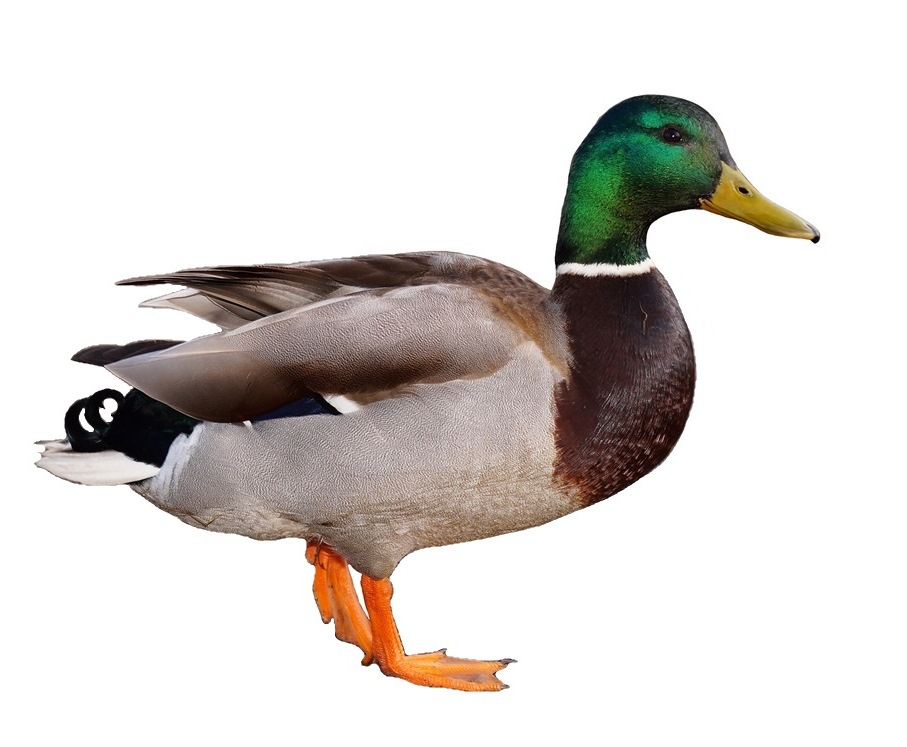
\includegraphics{images/Duck.png}

}

\caption{This is a duck. If Helena is reading this, yes it has a
creative commons licence.}

\end{figure}%

There are some cool new Quarto features making it easy to combine
multiple images. For example, we can add two ducks and specify we want
them in two columns.

\begin{Shaded}
\begin{Highlighting}[]
\SpecialCharTok{:::}\NormalTok{ \{}\CommentTok{\#fig{-}duck layout{-}ncol=2\}}
\SpecialCharTok{!}\NormalTok{[](images}\SpecialCharTok{/}\NormalTok{images}\SpecialCharTok{/}\NormalTok{Duck.png)}
\SpecialCharTok{!}\NormalTok{[](images}\SpecialCharTok{/}\NormalTok{images}\SpecialCharTok{/}\NormalTok{Duck.png)}
\NormalTok{Duck }\DecValTok{1}\NormalTok{ (left) and Duck }\DecValTok{2}\NormalTok{ (right). }
\SpecialCharTok{:::}
\end{Highlighting}
\end{Shaded}

\begin{figure}

\begin{minipage}{0.50\linewidth}
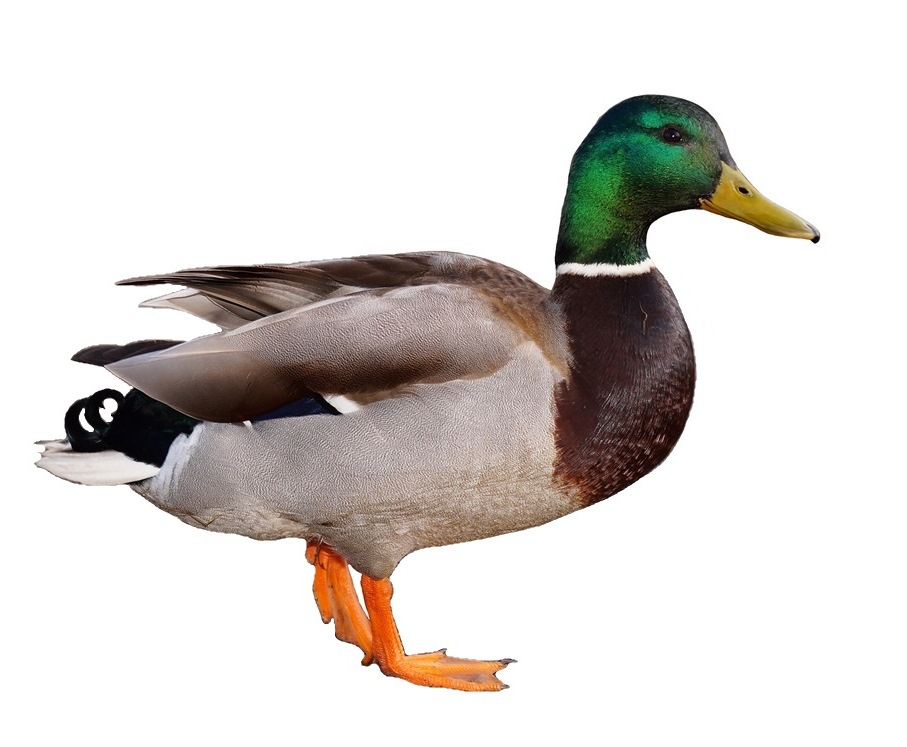
\includegraphics{images/Duck.png}\end{minipage}%
%
\begin{minipage}{0.50\linewidth}
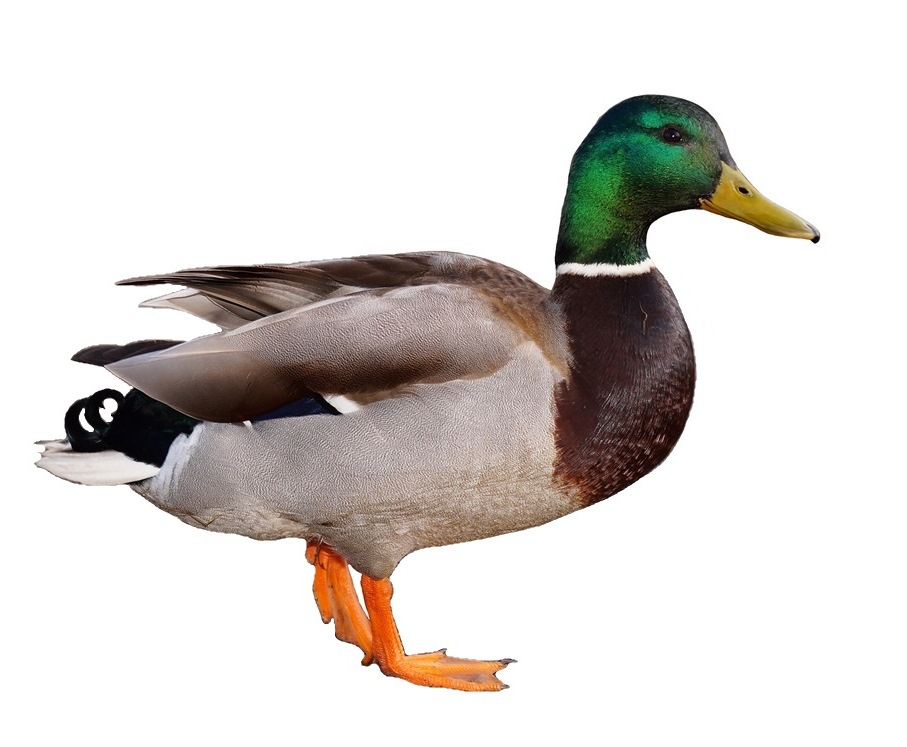
\includegraphics{images/Duck.png}\end{minipage}%

\caption{\label{fig-duck}Duck 1 (left) and Duck 2 (right).}

\end{figure}%

You can also reference figures to add little hyperlinks and
automatically number them. The title after the hash must start with
\texttt{fig} to be registered as a figure, and you can also add
\texttt{tbl} to number tables separately.

Figure~\ref{fig-duck} showed two ducks side by side. You do not even
need to type Figure: \texttt{@fig-duck}.

You can also use \texttt{knitr} to add figures, and using code chunks
has some new handy features using tags. They work in a similar way to
code options, but make it easier to add longer captions etc, as shown in
Figure~\ref{fig-img-duck}.

\begin{Shaded}
\begin{Highlighting}[]
\InformationTok{\textasciigrave{}\textasciigrave{}\textasciigrave{}\{r\}}
\InformationTok{\#| label: fig{-}img{-}duck}
\InformationTok{\#| fig.cap: "This is a longer caption about our beloved duck."}
\InformationTok{\#| fig{-}alt: "You can also add alt text to images."}

\InformationTok{knitr::include\_graphics("images/Duck.png")}
\InformationTok{\textasciigrave{}\textasciigrave{}\textasciigrave{}}
\end{Highlighting}
\end{Shaded}

\begin{figure}

\centering{

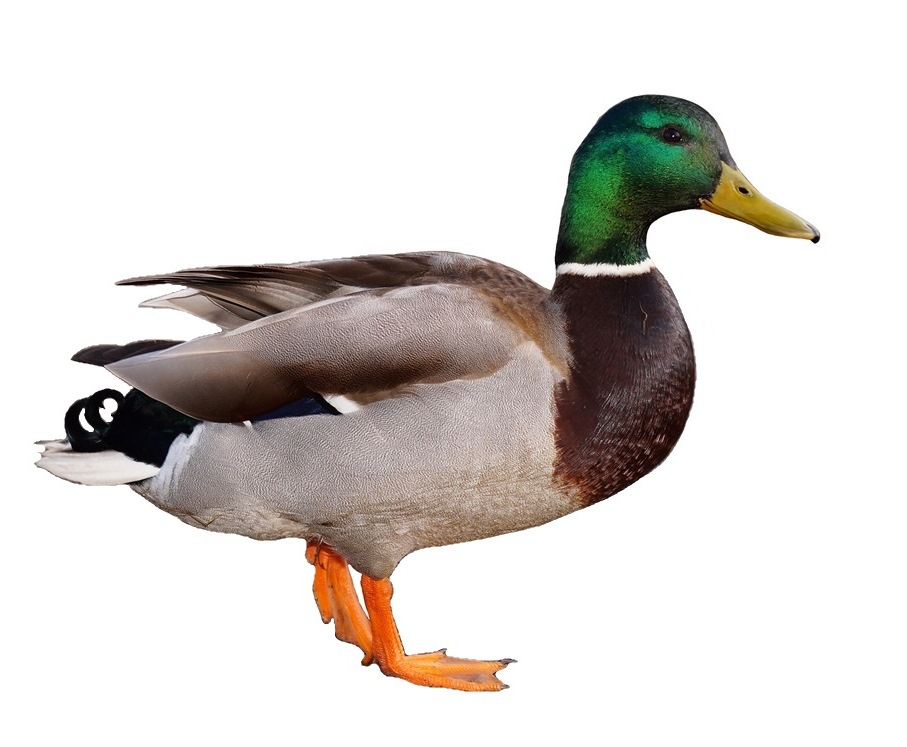
\includegraphics[width=3.02in,height=\textheight]{images/Duck.png}

}

\caption{\label{fig-img-duck}This is a longer caption about our beloved
duck.}

\end{figure}%

\subsection{Code chunks}\label{code-chunks}

If you are making a book to show code, there are a couple of features
that might be useful.

Adding code chunks will by default show both the code and output:

\begin{Shaded}
\begin{Highlighting}[]
\InformationTok{\textasciigrave{}\textasciigrave{}\textasciigrave{}\{r\}}
\InformationTok{rnorm(n = 5, mean = 10, sd = 2)}
\InformationTok{\textasciigrave{}\textasciigrave{}\textasciigrave{}}
\end{Highlighting}
\end{Shaded}

\begin{Shaded}
\begin{Highlighting}[]
\FunctionTok{rnorm}\NormalTok{(}\AttributeTok{n =} \DecValTok{5}\NormalTok{, }\AttributeTok{mean =} \DecValTok{10}\NormalTok{, }\AttributeTok{sd =} \DecValTok{2}\NormalTok{)}
\end{Highlighting}
\end{Shaded}

\begin{verbatim}
[1]  8.289999 10.208103 10.312386 12.155942  9.868879
\end{verbatim}

There are several features you can edit by adding different options. For
example, if you do not want to show the code, you can set
\texttt{echo=FALSE} after the r \texttt{\{r\ echo=FALSE\}}:

\begin{verbatim}
[1] 10.592479  9.019536  7.143294 10.018901 10.861884
\end{verbatim}

If you want to demonstrate code but not execute it - such as to
demonstrate inaccurate code, you can set \texttt{eval=FALSE} after the r
\texttt{\{r\ eval=FALSE\}}:

\begin{Shaded}
\begin{Highlighting}[]
\FunctionTok{rnorm}\NormalTok{(}\AttributeTok{n =} \DecValTok{5}\NormalTok{, }\AttributeTok{mean =} \DecValTok{10}\NormalTok{, }\AttributeTok{sd =} \DecValTok{2}\NormalTok{)}
\end{Highlighting}
\end{Shaded}

\subsection{Callout blocks}\label{callout-blocks}

My personal favourite features, you can highlight content with callout
blocks. These range from notes that people might find interesting, to
warnings that something could go mortally wrong.

\begin{Shaded}
\begin{Highlighting}[]
\SpecialCharTok{:::}\NormalTok{ \{.callout}\SpecialCharTok{{-}}\NormalTok{note\}}
\NormalTok{These are notes.}
\SpecialCharTok{:::}
\end{Highlighting}
\end{Shaded}

\begin{tcolorbox}[enhanced jigsaw, colbacktitle=quarto-callout-note-color!10!white, titlerule=0mm, leftrule=.75mm, title=\textcolor{quarto-callout-note-color}{\faInfo}\hspace{0.5em}{Note}, breakable, bottomrule=.15mm, opacitybacktitle=0.6, rightrule=.15mm, opacityback=0, arc=.35mm, colframe=quarto-callout-note-color-frame, toptitle=1mm, bottomtitle=1mm, toprule=.15mm, left=2mm, colback=white, coltitle=black]

These are notes.

\end{tcolorbox}

You can change the title by using hashes within the callout. They count
as real headers in the Quarto outline. So, if you use one hash, it looks
like a level one header which deeply disturbs me, so I like to use four
hashes to make more sense in the chapter structure.

\begin{Shaded}
\begin{Highlighting}[]
\SpecialCharTok{:::}\NormalTok{ \{.callout}\SpecialCharTok{{-}}\NormalTok{note\}}
\DocumentationTok{\#\#\#\# Look at my interesting title}
\NormalTok{These are notes.}
\SpecialCharTok{:::}
\end{Highlighting}
\end{Shaded}

\begin{tcolorbox}[enhanced jigsaw, colbacktitle=quarto-callout-note-color!10!white, titlerule=0mm, leftrule=.75mm, title=\textcolor{quarto-callout-note-color}{\faInfo}\hspace{0.5em}{Look at my interesting title}, breakable, bottomrule=.15mm, opacitybacktitle=0.6, rightrule=.15mm, opacityback=0, arc=.35mm, colframe=quarto-callout-note-color-frame, toptitle=1mm, bottomtitle=1mm, toprule=.15mm, left=2mm, colback=white, coltitle=black]

These are notes.

\end{tcolorbox}

You can also make the box collapse by default, which can be handy to
hide solutions or obscure tangents.

\begin{Shaded}
\begin{Highlighting}[]
\SpecialCharTok{:::}\NormalTok{ \{.callout}\SpecialCharTok{{-}}\NormalTok{note collapse}\OtherTok{=}\NormalTok{true\}}
\DocumentationTok{\#\#\#\# Please look at me}
\NormalTok{Secret secret notes. }
\SpecialCharTok{:::}
\end{Highlighting}
\end{Shaded}

\begin{tcolorbox}[enhanced jigsaw, colbacktitle=quarto-callout-note-color!10!white, titlerule=0mm, leftrule=.75mm, title=\textcolor{quarto-callout-note-color}{\faInfo}\hspace{0.5em}{Please look at me}, breakable, bottomrule=.15mm, opacitybacktitle=0.6, rightrule=.15mm, opacityback=0, arc=.35mm, colframe=quarto-callout-note-color-frame, toptitle=1mm, bottomtitle=1mm, toprule=.15mm, left=2mm, colback=white, coltitle=black]

Secret secret notes.

\end{tcolorbox}

Other types of callout blocks include:

\begin{itemize}
\tightlist
\item
  Warning
\end{itemize}

\begin{Shaded}
\begin{Highlighting}[]
\SpecialCharTok{:::}\NormalTok{ \{.callout}\SpecialCharTok{{-}}\NormalTok{warning\}}
\NormalTok{These are warnings.}
\SpecialCharTok{:::}
\end{Highlighting}
\end{Shaded}

\begin{tcolorbox}[enhanced jigsaw, colbacktitle=quarto-callout-warning-color!10!white, titlerule=0mm, leftrule=.75mm, title=\textcolor{quarto-callout-warning-color}{\faExclamationTriangle}\hspace{0.5em}{Warning}, breakable, bottomrule=.15mm, opacitybacktitle=0.6, rightrule=.15mm, opacityback=0, arc=.35mm, colframe=quarto-callout-warning-color-frame, toptitle=1mm, bottomtitle=1mm, toprule=.15mm, left=2mm, colback=white, coltitle=black]

These are warnings.

\end{tcolorbox}

\begin{itemize}
\tightlist
\item
  Important
\end{itemize}

\begin{Shaded}
\begin{Highlighting}[]
\SpecialCharTok{:::}\NormalTok{ \{.callout}\SpecialCharTok{{-}}\NormalTok{important\}}
\NormalTok{This is something important.}
\SpecialCharTok{:::}
\end{Highlighting}
\end{Shaded}

\begin{tcolorbox}[enhanced jigsaw, colbacktitle=quarto-callout-important-color!10!white, titlerule=0mm, leftrule=.75mm, title=\textcolor{quarto-callout-important-color}{\faExclamation}\hspace{0.5em}{Important}, breakable, bottomrule=.15mm, opacitybacktitle=0.6, rightrule=.15mm, opacityback=0, arc=.35mm, colframe=quarto-callout-important-color-frame, toptitle=1mm, bottomtitle=1mm, toprule=.15mm, left=2mm, colback=white, coltitle=black]

This is something important.

\end{tcolorbox}

\begin{itemize}
\tightlist
\item
  Tip
\end{itemize}

\begin{Shaded}
\begin{Highlighting}[]
\SpecialCharTok{:::}\NormalTok{ \{.callout}\SpecialCharTok{{-}}\NormalTok{tip\}}
\NormalTok{Here is a handy tip. }
\SpecialCharTok{:::}
\end{Highlighting}
\end{Shaded}

\begin{tcolorbox}[enhanced jigsaw, colbacktitle=quarto-callout-tip-color!10!white, titlerule=0mm, leftrule=.75mm, title=\textcolor{quarto-callout-tip-color}{\faLightbulb}\hspace{0.5em}{Tip}, breakable, bottomrule=.15mm, opacitybacktitle=0.6, rightrule=.15mm, opacityback=0, arc=.35mm, colframe=quarto-callout-tip-color-frame, toptitle=1mm, bottomtitle=1mm, toprule=.15mm, left=2mm, colback=white, coltitle=black]

Here is a handy tip.

\end{tcolorbox}

\begin{itemize}
\tightlist
\item
  And, a caution
\end{itemize}

\begin{Shaded}
\begin{Highlighting}[]
\SpecialCharTok{:::}\NormalTok{ \{.callout}\SpecialCharTok{{-}}\NormalTok{caution\}}
\NormalTok{Here is a caution about something.}
\SpecialCharTok{:::}
\end{Highlighting}
\end{Shaded}

\begin{tcolorbox}[enhanced jigsaw, colbacktitle=quarto-callout-caution-color!10!white, titlerule=0mm, leftrule=.75mm, title=\textcolor{quarto-callout-caution-color}{\faFire}\hspace{0.5em}{Caution}, breakable, bottomrule=.15mm, opacitybacktitle=0.6, rightrule=.15mm, opacityback=0, arc=.35mm, colframe=quarto-callout-caution-color-frame, toptitle=1mm, bottomtitle=1mm, toprule=.15mm, left=2mm, colback=white, coltitle=black]

Here is a caution about something.

\end{tcolorbox}

\subsection{References}\label{references}

If you want to add proper references instead of just hyperlinks, you
need a .bib file from a reference manager.

The .bib file should be in the include folder (unless you point it
somewhere else) and you can specify it in the \texttt{\_quarto.yml} file
through the bibliography entry:

\begin{Shaded}
\begin{Highlighting}[]
\NormalTok{bibliography}\SpecialCharTok{:}\NormalTok{ include}\SpecialCharTok{/}\NormalTok{references.bib}
\end{Highlighting}
\end{Shaded}

\begin{tcolorbox}[enhanced jigsaw, colbacktitle=quarto-callout-tip-color!10!white, titlerule=0mm, leftrule=.75mm, title=\textcolor{quarto-callout-tip-color}{\faLightbulb}\hspace{0.5em}{How do I download and edit a .bib file?}, breakable, bottomrule=.15mm, opacitybacktitle=0.6, rightrule=.15mm, opacityback=0, arc=.35mm, colframe=quarto-callout-tip-color-frame, toptitle=1mm, bottomtitle=1mm, toprule=.15mm, left=2mm, colback=white, coltitle=black]

I use Zotero as a reference manager and its super easy to download a
.bib file for a project you are working on. Downloading one entry is a
little annoying as you need to export it as BibTex and copy from the
file it produces, but if you create a folder to store everything for the
book, you can just export the folder each time you add new entries
(\texttt{right\ click\ \textgreater{}\textgreater{}\ export\ collection\ \textgreater{}\textgreater{}\ BibTex\ format\ and\ OK}).

If you do have the single entry, you can open the .bib file within
RStudio and copy the entry in. It will look something like this:

\begin{Shaded}
\begin{Highlighting}[]
\SpecialCharTok{@}\NormalTok{article\{bartlett\_power\_2022,}
\NormalTok{    title }\OtherTok{=}\NormalTok{ \{Power to the \{People\}}\SpecialCharTok{:}\NormalTok{ \{A\} \{Beginner\}’s \{Tutorial\} to \{Power\} \{Analysis\} using jamovi\},}
\NormalTok{    volume }\OtherTok{=}\NormalTok{ \{}\DecValTok{6}\NormalTok{\}}
\NormalTok{    ...\}}
\end{Highlighting}
\end{Shaded}

which stores all the information for the \texttt{.csl} to pull out and
cite/reference as needed.

\end{tcolorbox}

To cite, you need the code at the start of the bib entry. For example,
\texttt{@bartlett\_power\_2022} produces Bartlett \& Charles (2022) and
the full reference will be added to the references chapter.

Depending on the citation style you want, there are different codes,
such as adding it in parentheses \texttt{{[}@bartlett\_power\_2022{]}}
(Bartlett \& Charles, 2022). For a full list of options, you can check
out the \href{https://quarto.org/docs/authoring/citations.html}{Quarto
citation guide}.

By default, the book template has APA style for referencing, but if you
need a different referencing style, you can add and specify a different
.csl file within \texttt{\_quarto.yml}.

\begin{Shaded}
\begin{Highlighting}[]
\NormalTok{csl}\SpecialCharTok{:}\NormalTok{ include}\SpecialCharTok{/}\NormalTok{apa.csl}
\end{Highlighting}
\end{Shaded}

\begin{tcolorbox}[enhanced jigsaw, colbacktitle=quarto-callout-tip-color!10!white, titlerule=0mm, leftrule=.75mm, title=\textcolor{quarto-callout-tip-color}{\faLightbulb}\hspace{0.5em}{How do I specify a .csl file?}, breakable, bottomrule=.15mm, opacitybacktitle=0.6, rightrule=.15mm, opacityback=0, arc=.35mm, colframe=quarto-callout-tip-color-frame, toptitle=1mm, bottomtitle=1mm, toprule=.15mm, left=2mm, colback=white, coltitle=black]

\texttt{.csl} stands for citation style language and you can download
one from the \href{https://www.zotero.org/styles}{Zotero style
repository}. For example, you could search for vancouver, click on the
link, and it will download a new .csl file you can add to your
repository within \texttt{include/}.

\end{tcolorbox}

\subsection{\texorpdfstring{\texttt{webexercises} interactive
questions}{webexercises interactive questions}}\label{webexercises-interactive-questions}

The book template automatically includes the \texttt{webexercises}
package which can add interactive questions for self-tests. This is
great for students checking their understanding through MCQs or adding
easy to check answers like numbers.

\subsubsection{MCQs}\label{mcqs}

You can add questions through inline code, or by first specifying them
in an R code block if it makes it easier to edit longer text.

For example, this workshop is:

\begin{itemize}
\tightlist
\item
  \begin{enumerate}
  \def\labelenumi{(\Alph{enumi})}
  \tightlist
  \item
    Life changing\\
  \end{enumerate}
\item
  \begin{enumerate}
  \def\labelenumi{(\Alph{enumi})}
  \setcounter{enumi}{1}
  \tightlist
  \item
    Boring\\
  \end{enumerate}
\item
  \begin{enumerate}
  \def\labelenumi{(\Alph{enumi})}
  \setcounter{enumi}{2}
  \tightlist
  \item
    Mediocre\\
  \end{enumerate}
\item
  \begin{enumerate}
  \def\labelenumi{(\Alph{enumi})}
  \setcounter{enumi}{3}
  \tightlist
  \item
    OK
  \end{enumerate}
\end{itemize}

\begin{Shaded}
\begin{Highlighting}[]
\StringTok{\textasciigrave{}}\AttributeTok{r longmcq(c(answer = "Life changing", "Boring", "Mediocre", "OK"))}\StringTok{\textasciigrave{}} 
\end{Highlighting}
\end{Shaded}

\subsubsection{Single answer}\label{single-answer}

You can ask simple single answers that are easy to evaluate:

\begin{itemize}
\tightlist
\item
  On a scale of 1 (very dissatisfied) - 7 (very satisfied), how pleased
  are you with this workshop? \_
\end{itemize}

\begin{Shaded}
\begin{Highlighting}[]
\StringTok{\textasciigrave{}}\AttributeTok{r fitb(7)}\StringTok{\textasciigrave{}}
\end{Highlighting}
\end{Shaded}

\subsubsection{True or false}\label{true-or-false}

If you want an even simpler response, you can ask true or false.

\begin{itemize}
\tightlist
\item
  After the workshop, I am going to make my own book: TRUE / FALSE
\end{itemize}

\begin{Shaded}
\begin{Highlighting}[]
\StringTok{\textasciigrave{}}\AttributeTok{r torf(TRUE)}\StringTok{\textasciigrave{}}
\end{Highlighting}
\end{Shaded}

\subsection{Embedding files to
download}\label{embedding-files-to-download}

Using a similar format to creating hyperlinks, you can embed files for
people to download and use in the chapter. This can be really useful for
student activities as you can give them a data set to follow along to
your tutorials with.

First, you need to add a file within your book directory. If you have
loads of data or files across your book, you might want a separate
folder (I call mine \texttt{data} or \texttt{supporting}), but I have
put a simple .csv in the \texttt{include/} folder.

If you click on \href{include/test_data.csv}{.csv file}, it will
download to your browser or people might need to right click and ``save
link as''. It follows the same format as hyperlinks:

\begin{Shaded}
\begin{Highlighting}[]
\NormalTok{click on [.csv file](include}\SpecialCharTok{/}\NormalTok{test\_data.csv)}
\end{Highlighting}
\end{Shaded}

\subsection{Adding a glossary}\label{adding-a-glossary}

Another cool feature that Lisa created is adding a glossary of terms.
\texttt{glossary} is its own R package, but by default \texttt{booktem}
includes it. You have two options, you can either add your own
definitions as you go along, or if you are teaching data skills, you can
use the \href{https://psyteachr.github.io/glossary/}{PsyTeachR
glossary}.

\begin{tcolorbox}[enhanced jigsaw, colbacktitle=quarto-callout-important-color!10!white, titlerule=0mm, leftrule=.75mm, title=\textcolor{quarto-callout-important-color}{\faExclamation}\hspace{0.5em}{Important}, breakable, bottomrule=.15mm, opacitybacktitle=0.6, rightrule=.15mm, opacityback=0, arc=.35mm, colframe=quarto-callout-important-color-frame, toptitle=1mm, bottomtitle=1mm, toprule=.15mm, left=2mm, colback=white, coltitle=black]

You still need to add definitions for anything that is not included in
the PsyTeachR glossary. If you try and render and the item does not
exist, you will get an error and you will need to manually add the
definition within the inline code.

\end{tcolorbox}

There are two main components to creating a glossary. First, you need to
add glossary items as you work through your chapter using inline code.
For example, I might want to define what a glossary{An alphabetical list
of words with explanations.} is:

\begin{Shaded}
\begin{Highlighting}[]
\StringTok{\textasciigrave{}}\AttributeTok{r glossary("glossary", def = "An alphabetical list of words with explanations.")}\StringTok{\textasciigrave{}}
\end{Highlighting}
\end{Shaded}

If you hover or click on the text, you will see the definition appear.
There are different settings for this, so make sure you check the
\href{https://debruine.github.io/glossary/articles/glossary.html}{glossary
documentation}.

At the end of each chapter, you can then include a glossary table which
shows all the words you used in the chapter. Just make sure you add
\texttt{echo=FALSE} to the code chunk, so that the function does not
appear.

\begin{Shaded}
\begin{Highlighting}[]
\InformationTok{\textasciigrave{}\textasciigrave{}\textasciigrave{}\{r\}}
\InformationTok{glossary\_table()}
\InformationTok{\textasciigrave{}\textasciigrave{}\textasciigrave{}}
\end{Highlighting}
\end{Shaded}

This produces:

\begin{longtable*}[t]{ll}
\toprule
term & definition\\
\midrule
glossary & An alphabetical list of words with explanations.\\
\bottomrule
\end{longtable*}

The behaviour of glossary table and whether you use all your own
definitions or point to the PsyTeachR glossary is controlled by some R
code in the \texttt{booktem} files. It will be easier to point out in
the workshop, but you are looking for \texttt{R/my\_setup.R}.

You can add definitions as you go along with inline code, or you can
create and edit a .yml file for your terms if you would prefer to edit
that way. See the \texttt{glossary} documentation for more information.

\bookmarksetup{startatroot}

\chapter*{References}\label{references-1}
\addcontentsline{toc}{chapter}{References}

\markboth{References}{References}

\phantomsection\label{refs}
\begin{CSLReferences}{1}{0}
\bibitem[\citeproctext]{ref-bartlett_power_2022}
Bartlett, J., \& Charles, S. (2022). Power to the {People}: {A}
{Beginner}'s {Tutorial} to {Power} {Analysis} using jamovi.
\emph{Meta-Psychology}, \emph{6}.
\url{https://doi.org/10.15626/MP.2021.3078}

\end{CSLReferences}



\end{document}
